\chapter{Studium przypadku}
\par W tym rozdziale poświęconym na studium przypadku, zostanie przeprowadzony eksperyment oparty o wcześniej krótko opisany model optymalizacyjny. Jednocześnie, ten rozdział pokaże pełen proces tworzenia modelu optymalizacyjnego w oparciu o zadany problem oraz jego implementacje w wybranym środowisku. Głównym celem tego eksperymentu jest praktyczne zastosowanie teoretycznych założeń modelu optymalizacyjnego oraz zweryfikowanie jego skuteczności w rzeczywistych warunkach. 
\par Do eksperymentu zostaną wykorzystane dane wygenerowane przez skrypt \verb|generator.py|, który wyprodukuje losowe dane, odzwierciedlające różne scenariusze panujące w firmach IT. Tak wygenerowane dane zostaną użyte jako dane wejściowe dla skryptu \verb|optimizer.py|, który przeprowadzi właściwą optymalizacje składu zespołu projektowego. Optymalizacja będzie mieć na celu uzyskanie takiego zestawu pracowników, który jednocześnie spełnia ograniczenia budżetowe oraz ograniczenia minimalnej sumy umiejętności członków tego zespołu.
\par Dane pozyskane poprzez uruchomienie obu skryptów zostaną poddane analizie statystycznej, której wyniki zostaną dokładnie omówione i przedstawione. Celem analizy będzie zawarcie oceny różnych parametrów takich jak średnia, mediana, odchylenie standardowe, maksimum oraz minimum poszczególnych umiejętności, jak i wynagrodzeń.  Wyniki analiz zostaną dokładnie omówione oraz przedstawione w tabelach oraz na wykresach, co umożliwi bardziej przejrzyste zrozumienie wyników optymalizacji.
\par Na koniec rozdziału zostaną omówione możliwe wady, ograniczenia oraz wyzwania związane z zastosowanym modelem optymalizacyjnym. Przykładowymi mogą być uproszczony model oceny umiejętności pracowników lub brak pełnej reprezentacji rzeczywistych scenariuszy. Zidentyfikowanie tych wad i ograniczeń, może znacząco usprawnić przebieg przyszłych eksperymentów oraz może prowadzić do przyszłych usprawnień modelu.
\par W literaturze istnieje wiele badań na temat zastosowań programowania liniowego oraz badań operacyjnych (ang. Operations Research lub OR) w optymalizacji zarządzania projektami. Przykładem może być praca L. V. Tavares, który pisze "\textit{Badania operacyjne wniosły istotne naukowe wkłady w sukces zarządzania projektami, nie tylko poprzez różnorodne modele pozwalające zrozumieć i przedstawiać projekty, ale także dzięki opracowaniu algorytmów i narzędzi wspierających rolę decyzyjną kierownika projektu.}" \parencite{tavares2002review}. Potwierdza tym znaczenie badań operacyjnych i programowania liniowego w dziedzinie zarządzania projektami,a co za tym idzie zespołami projektowymi. Dzięki temu, zastosowanie OR i LP dla tego eksperymentu jest w pełni uzasadnione i można oczekiwać realnie użytecznych wyników i wniosków.

\section{Zadanie optymalizacyjne jako studium przypadku} \label{sec:studium}
\par W celu zaprezentowania użyteczności wcześniej przedstawionego modelu optymalizacyjnego oraz skryptu służącego do jej przeprowadzania, zostało sporządzone zadanie optymalizacyjne. Zadanie przedstawia problem optymalizacyjny, do którego rozwiązania posłuży wyżej wymieniony model oraz skrypt. Problem zadania polega na minimalizacji kosztów zespołu projektowego w firmie IT, odpowiedzialnego za wykonanie pewnego oprogramowania. Przy minimalizacji kosztów zespołu, muszą być brane pod uwagę ograniczenia w formie budżetu przeznaczonego na projekt oraz jak najwyższej łącznej oceny umiejętności zespołu. Aby zapewnić przejrzyste oraz poprawne wykonanie zadania, problem należy podzielić na części. Oznacza to wcześniejsze wypisanie parametrów i zmiennych decyzyjnych, określenia ograniczeń na ich podstawie oraz wyznaczenia funkcji celu. Te czynności poprzedzają implementacje modelu optymalizacyjnego w środowisku języka Python lub w innym wybranym środowisku (np. środowisko R, MatLab itp.).

    \subsection{Definicja problemu}\label{subsec:problem}
    \par Menedżer projektu ma za zadanie skompletować optymalny zespół pod nowy projekt, którym będzie zajmować się firma. Ma do dyspozycji plik z danymi o pracownikach (\verb|pracownicy.csv|), w którym znajdują się dane o każdym z pracowników. W całej firmie jest 2000 pracowników, którzy mogliby należeć do tego zespołu. Dane przedstawiają poszczególne umiejętności, sumę umiejętności oraz żądane wynagrodzenia na godzinę. Każda z umiejętności jest zapisana jako liczba całkowita z przedziału od 0 do 1, a wynagrodzenia uzależnione jest od wartości sumy umiejętności. Umiejętności podzielone zostały na 5 kategorii: \verb|umiejętności Angular|, \verb|umiejętności Java|, \verb|umiejętności UI/UX|, \verb|umiejętności SQL| oraz \verb|znajomość języka angielskeigo|. Przykładowe wiersze z pliku \verb|pracownicy.csv| wyglądają następująco:
    \begin{figure}[H]
        \centering
        \includegraphics[width=\linewidth]{chapters/Images/pracownicy_przykład.png}
        \cprotect\caption{Przykładowe dane pracowników w pliku \verb|pracownicy.csv|\\ Źródło:\textit{ opracowanie własne}} 
    \end{figure}

    \par Menedżer musi wziąć pod uwagę ograniczenia przy wyborze pracowników, do których należą budżet i minimalny poziom umiejętności zespołu potrzebny do wykonania projektu. Budżet został określony przez dyrektora firmy na 150 000 złotych, a czas na wykonanie projektu stanowi 120 roboczogodzin (dalej RBH). Dla uproszczenie zadania budżet bierze pod uwagę tylko wynagrodzenia pracowników. Z uwagi na złożoność i wymagania jakie stawia wytworzenie tego oprogramowania, menedżer ustalił, że minimalny poziom umiejętności w tym zespole będzie wynosić 85 punktów.
    \par Ręczne przeglądanie 2000 wierszy z danymi i sprawdzanie optymalności zajęłoby zbyt dużo czasu, stąd potrzeba na zastosowanie optymalizacji matematycznej, programowania liniowego i języka programowania Python. Następnymi krokami będzie wypisanie zmiennych i parametrów oraz wyznaczenie funkcji celu i określenie ograniczeń.

    \subsection{Parametry i zmienna decyzyjna}
    \par W tej części zostały wypisane zmienne i parametry, użyte w modelu optymalizacyjnym do wyznaczenia optymalnego składu zespołu projektowego.
    \begin{description}

        \item[Zbiór pracowników] - Zbiór wszystkich pracowników zawartych w pliku \verb|pracownicy.csv|: $\mathcal{P}$

        \item[Liczba pracowników] - Liczba wszystkich pracowników zawartych w pliku \verb|pracownicy.csv|: $n$
    
        \item[Budżet] - Całkowity budżet na wynagrodzenia pracowników: $B = 150 000pln$
        
        \item[Czas na wykonanie projektu] - Całkowita liczba RBH przeznaczona na projekt: $h = 120 RBH$

        \item[Umiejętności pracownika] - Wartość umiejętności $j$ u pracownika $i$ z zakresu $[0, 1]$: $Skill$

        \item[Zbiór umiejętności] - Zbiór wszystkich umiejętności wyróżnionych w tabeli w pliku \verb|pracownicy.csv|: $\mathcal{U}$

        \item[Liczba umiejętności] - Liczba wszystkich umiejętności wyróżnionych w tabeli w pliku \verb|pracownicy.csv|: $5$
        
        \item[Suma umiejętności pracownika] - Wartość sumy wszystkich umiejętności pracownika $i$: 
            \[
                \sum_{Skill \in \mathcal{U}}^{m} i_{Skill} = SumSkill
            \]
        
        \item[Wymagany poziom umiejętności] - minimalny wymagany poziom umiejętności w zespole: $req$
        
        \item[Minimalny poziom umiejętności zespołu] - Minimalna suma umiejętności wszystkich pracowników w zespole jest opisana wzorem:
        
        \[
        \sum_{i \in \mathcal{P}}^{n} SumSkill_{i} = Min_{SumSkill_{i}}
        \]
        
        gdzie \(SumSkill_{i}\) reprezentuje sumę umiejętności \(i\)-tego pracownika.
        
        \item[Koszt godzinowy pracownika] - Kwota wynagrodzenia na godzinę w złotówkach dla \(i\)-tego pracownika: \(K_{i}\)

        \item[Całkowity koszt pracownika] - Całkowita kwota wynagrodzenia za cały przebieg projektu dla \(i\)-tego pracownika: 
            \[
                K_{i} \cdot h
            \]

        \item[Zmienne decyzyjna] - Zmienne binarne określające przydzielenie pracownika do zespołu
            {\begin{itemize}
                \item $x_{i} = 1$ - jeśli pracownik został wybrany do zespołu
                \item $x_{i} = 0$ - jeśli pracownik nie został wybrany do zespołu
            \end{itemize}}
    \end{description}
    
    \subsection{Funkcja celu i ograniczenia}
    \par Po wyznaczeniu zmiennych decyzyjnych i parametrów potrzebnych do stworzenia modelu, należy wypisać ograniczenia oraz sporządzić funkcje celu. 

    \begin{description}
        \item[Ograniczenie budżetowe] Pierwszym z ograniczeń będzie ograniczenie budżetowe. W zadaniu było wyjaśnione, że łączny budżet na wynagrodzenia pracowników nie może przekroczyć 150 000 złotych. Takie ograniczenie, przy przyjętych oznaczeniach, można opisać wzorem:
            \[
                \sum_{i \in \mathcal{P}}^{n} (x_{i} \cdot K_{i} \cdot h) \leq B
            \]
        
        \item[Ograniczenie minimalnego poziomu umiejętności] Następnym ograniczeniem jest minimalny poziom umiejętności zespołu     $Min_{SumSkill_{i}}$, który przy przyjętych oznaczeniach można opisać wzorem:
            \begin{enumerate}
                \item 
                    \[
                        \sum_{i \in \mathcal{P}}^{n} \sum_{Skill \in \mathcal{U}}^{m} i_{Skill} \leq req
                    \]
                \item 
                    \[
                        \sum_{i \in \mathcal{P}}^{n} SumSkill \leq req
                    \]      
                \item 
                    \[
                        Min_{SumSkill_{i}} \leq req
                    \]
                \item 
                    \[
                        Min_{SumSkill_{i}} \leq 85
                    \] 
        \end{enumerate} 
        
        \item[Funkcja celu] Z treści problemu można wywnioskować, że celem optymalizacji zespołu projektowego będzie minimalizacja kosztów całego zespołu, przy jednoczesnym założeniu utrzymania jak najwyższego poziomu umiejętności zespołu. Z  tym wziętym pod uwagę i przy przyjętych oznaczeniach można wyznaczyć funkcje celu takim wzorem:
            \[
               Minimize \sum_{i \in \mathcal{P}}^{n} (x_{i} \cdot K_{i} \cdot h)
            \]
    \end{description}

    \par W tym podrozdziale zostało przedstawione zadanie optymalizacyjne w ramach studium przypadku. Owa optymalizacja została sformułowana jako minimalizacja kosztów zespołu projektowego w firmie IT, która dysponuje danymi o swoich pracownikach w pliku \verb|pracownicy.csv|. Zidentyfikowano kluczowe parametry i zmienne, a także określono funkcje celu oraz jej ograniczenia. Do ograniczeń należało ograniczenie budżetowe oraz ograniczenie minimalnego poziomu umiejętności zespołu, a funkcja celu dąży do minimalizacji kosztu zespołu. Implementacja tego zadania, a co za tym idzie modelu optymalizacyjnego, zostanie przeprowadzona w języku programowania Python z wykorzystaniem bibliotek \verb|PuLP| dla łatwego modelowania oraz \verb|Pandas| dla pracy z plikami csv. 
    
\section{Zastosowanie modelu do optymalizacji zespołu projektowego}
\par W tej części pracy zostanie przeprowadzone badanie problemu opisanego w sekcji \refnote{sec:studium}. Badanie będzie polegało na wygenerowaniu danych o pracownikach za pomocą \verb|generator.py|. Następnie zostanie przeprowadzona analiza wygenerowanych danych za pomocą skryptu \verb|analyzer.py|. Po przeprowadzonej analizie, wygenerowane dane zostaną załadowane do skryptu \verb|optimizer.py|, który dokona optymalizacji problemu, a jej wyniki również zostaną poddane analizę przez skrypt \verb|analyzer.py|. Analizę poprzedzi omówienie kodu analizującego dane, w celu wyjaśnienia działania i metodologii użytej przy analizie wyników.
    
    \subsection{Implementacja modelu optymalizacyjnego}\label{subsec:optimizer_implementacja}
        \par W tej sekcji została szczegółowo omówiona implementacja modelu optymalizacyjnego, który pozwala na efektywne zarządzanie zasobami ludzkimi w firmie IT, z wykorzystaniem technik programowania liniowego. Implementacja ta obejmuje różnorodne narzędzia i technologie, które umożliwiają budowę, rozwiązanie oraz analizę wyników modelu optymalizacyjnego.
    
    \subsubsection{Opis wykorzystanych narzędzi i technologii}
    \par W celu implementacji modelu optymalizacyjnego, zastosowano kilka kluczowych narzędzi i technologii. Każde z tych narzędzi odgrywa istotną rolę w procesie budowy, rozwiązania oraz analizy modelu programowania liniowego. W niniejszej sekcji omówione zostaną najważniejsze z nich.
    \begin{description}
        
        \item[Python] - Python jest językiem programowania wysokiego poziomu, który jest szeroko stosowany w analizie danych, uczeniu maszynowym oraz optymalizacji. Jego prostota i czytelność, w połączeniu z bogatym ekosystemem bibliotek, czynią go idealnym wyborem do realizacji zadań związanych z optymalizacją. Jak podkreśla \parencite{lutz2013learning} w swojej książce, Python jest doskonałym narzędziem dla inżynierów danych ze względu na swoją wszechstronność i dostępność bibliotek wspierających złożone analizy.
        
        \item[Pandas] - Biblioteka pandas jest jednym z najważniejszych narzędzi w ekosystemie Pythona, umożliwiającym łatwe i efektywne przetwarzanie oraz analizę danych. Pandas oferuje struktury danych takie jak DataFrame, które są niezwykle użyteczne w manipulacji dużymi zestawami danych. Twórca Pandas, \parencite{mckinney2013python}, opisuje bibliotekę jako narzędzie, które radykalnie zmienia sposób, w jaki analitycy pracują z danymi, umożliwiając szybkie i intuicyjne operacje na dużych zestawach danych. W niniejszym projekcie pandas jest używane do wczytywania danych pracowników z pliku CSV, ich transformacji oraz przygotowania do dalszej analizy i modelowania.
        
        \item[PuLP] - Jest to biblioteka Python'a do modelowania problemów programowania liniowego. Umożliwia definiowanie zmiennych decyzyjnych, funkcji celu oraz ograniczeń w sposób deklaratywny, a następnie rozwiązywanie tych problemów za pomocą różnych solverów. W tym studium przypadku, PuLP jest wykorzystywane do stworzenia i rozwiązania modelu optymalizacyjnego, który minimalizuje koszty zatrudnienia przy jednoczesnym spełnieniu wymagań dotyczących umiejętności zespołu. Jak wskazuje, Mitchell S. \parencite{mitchell2009introduction}, obszar badań operacyjnych w którym biblioteka PuLP jest przydatna to rozwój i modelowanie problemów LP.
        
        \item[CSV] - Format CSV (Comma-Separated Values) jest powszechnie używany do przechowywania i wymiany danych w formacie tekstowym. W projekcie dane wejściowe pracowników są wczytywane z pliku CSV, a wyniki optymalizacji również zapisywane są w tym formacie, co ułatwia ich późniejszą analizę i interpretację. Format CSV jest prosty i szeroko kompatybilny, co czyni go idealnym wyborem do pracy z danymi w różnych etapach procesu optymalizacji.
        
        \item[Integracja] - Wszystkie te narzędzia i technologie są zintegrowane w celu stworzenia kompletnego systemu optymalizacji. Python, wraz z bibliotekami \verb|pandas| i \verb|PuLP|, umożliwia efektywne przetwarzanie danych, modelowanie problemów programowania liniowego oraz znajdowanie optymalnych rozwiązań. Format CSV zapewnia prosty sposób wymiany danych między różnymi etapami procesu optymalizacji, co ułatwia pracę nad danymi i ich analizę. Dzięki temu możliwe jest stworzenie efektywnego i łatwego w użyciu narzędzia do zarządzania zasobami ludzkimi w firmach IT.
        
    \end{description}
        
    \subsubsection{Omówienie kodu źródłowego modelu optymalizacyjnego}
    \par W tej sekcji rozdziału zostanie szczegółowo omówiony kod źródłowy skryptu optymalizacyjnego, którego celem jest optymalizacja składu zespołu projektowego w firmie IT. Dane pracowników wykorzystane do optymalizacji zostają pobierane z pliku \verb|pracownicy.csv| a następnie zostają wczytane do modelu w celu optymalizacji. Model posiada implementacje ograniczeń opisanych w problemie oraz wyznaczonej funkcji celu, a także zapisuje wyniki optymalizacji w pliku \verb|wybrani_pracownicy.csv| w celu dalszej analizy.

    \lstinputlisting[language=Python, caption={Kod źródłowy modelu. \\Źródło:\textit{ opracowanie własne}}]{optimizer.py}

    \begin{description}
        \item[Linie 1-2] W tych dwóch liniach importowane są biblioteki niezbędne do realizacji modelu optymalizacyjnego, które szczegółowo zostały omówione w poprzednim rozdziale. W środowisku języka \verb|Python|, potrzeba i chęć wykorzystania konkretnej biblioteki wiąże się z jej wcześniejszym zaimportowaniem.
        \item[Linie 4-5] W liniach 4 i 5 skrypt pyta użytkownika o nazwę pliku z danymi pracowników przeznaczonych do optymalizacji (zmienna \verb|sciezka_do_pliku|) oraz o nazwę pliku, który służy do przechowania wyników optymalizacji (zmienna \verb|nazwa_pliku_csv|).
        \item[Linie 9-11] W tych liniach użytkownik jest proszony o podanie wartości dla zmiennych \verb|budzet, liczba_godzin_projektu| oraz \verb|minimalne_umiejetnosci|. Te trzy linie są kluczowe dla powodzenia optymalizacji, gdyż na ich podstawie są ustalane ograniczenia.
        \item[Linie 13-14] Następnie jest tworzony nowy problem optymalizacyjny nazwany \verb|Optymalizacja_zespolu_projektowego|, który będzie dążyć do minimalizacji łącznego kosztu zespołu. Po utworzeniu modelu, jest zdefiniowana zmienna binarna \verb|x_{i}| służąca do określenia, czy pracownik został wybrany do zespołu (wartość 1), czy też nie został wybrany do zespołu (wartość 0).
        \item[Linie 16-19] W linii 16 definiowana jest funkcja celu opisana wcześniej, definiująca całkowity koszt jako sumę wynagrodzeń pracowników. Następnie dodawane są ograniczenia budżetowe oraz minimalnego poziomu umiejętności opisane we wcześniejszych sekcjach. Ograniczenie budżetowe oblicza łączny koszt wynagrodzeń i zapewnia, że jest mniejsze lub równe założonemu budżetowi. Minimalna suma umiejętności natomiast, czy suma umiejętności wybranych pracowników jest większa lub równa założonemu poziomowi. Następnie model jest rozwiązywany za pomocą metody \verb|solve()|.
        \item[Linie 21-24] W tych liniach, po zakończonej optymalizacji, pobierane są informacje na temat statusu modelu (\verb|status|), o indeksach wybranych pracowników (\verb|wybrani_pracownicy_indeksy|) oraz łącznego kosztu po optymalizacji (\verb|laczny_koszt|).
        \item[Linie 26-36] Te linie zwracają informacje w formie tekstowej na temat statusu modelu, listę wybranych pracowników i ich ilości, imiona wybranych pracowników oraz informacje o łącznym koszcie. Na koniec, skrypt zapisuje uzyskane wyniki do pliku .csv o podanej wcześniej przez użytkownika nazwie. Struktura danych w pliku zawierającym wyniki prezentuje się w następujący sposób: 
            \begin{figure}[H]
                \centering
                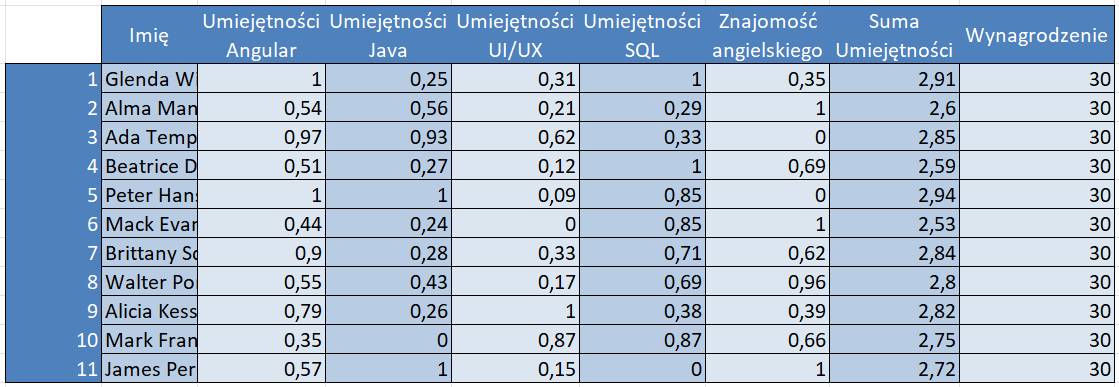
\includegraphics[width=\linewidth]{chapters/Images/wybrani_pracownicy_przyklad_csv.png}
                \cprotect\caption{Przykładowe dane w pliku \verb|wybrani_praocwnicy.csv|\\ Źródło:\textit{ opracowanie własne}}
            \end{figure}
    \end{description}
    
    \par W ten sposób kod realizuje zadanie optymalizacji składu zespołu projektowego, minimalizując koszty przy jednoczesnym spełnieniu wymagań dotyczących umiejętności i budżetu. W następnych sekcjach tego rozdziału zostanie przeprowadzona dokładna analiza statystyczna danych wszystkich pracowników jak i wyników po przeprowadzonej optymalizacji, która posłuży do wyciągnięcia wniosków. Dzięki analizie będzie można określić wady oraz zalety modelu, a także jego użyteczność w bardziej rzeczywistych scenariuszach.

    \subsection{Generacja danych o pracownikach}\label{sec:generacja_danych}
    \par Generowanie danych o pracownikach jest istotnym etapem w testowaniu modelu optymalizacyjnego i przeprowadzania symulacji. Skrypt \verb|generator.py|, opisany w sekcji \refnote{sec:kod_generator}, pozwala na szybkie i efektywne tworzenie losowych danych, które będą używane w dalszych analizach. Korzystanie z losowo generowanych danych umożliwia elastyczne testowanie różnych scenariuszy i pozwala sprawdzić wszechstronność modelu.
    
    \par Przed wygenerowaniem danych, należy upewnić się, że system posiada odpowiednie wymagania programowe. Do takowych należą:
    \begin{description}
        \item[System operacyjny] Windows, macOS lub Linux
        \item[Python] Wersja języka Python 3.11 lub nowsza 
    \end{description}
    Dodatkowo, należy zainstalować biblioteki wymagane do działania skryptu:
    \begin{itemize}
        \item Pandas
        \item NumPy
        \item Names
    \end{itemize}
    
    \lstinputlisting[language=bash, firstline=5, lastline=5, caption=Komenda instalacji bibliotek dla skryptu generatora danych \\Źródło:\textit{ opracowanie własne}]{snippets.sh}
    
    \par Aby wygenerować dane, koniecznym jest podanie kilku znaczących parametrów, takich jak liczba pracowników oraz średnia i odchylenie standardowe, które zostaną użyte w rozkładzie normalnym. W tym badaniu przyjęto następujące wartości:
    
    \begin{itemize}
        \item \verb|liczba_pracowników = 2000|
        \item \verb|srednia_umiejetnosci = 0.4|
        \item \verb|odchylenie_standardowe = 0.5|
    \end{itemize}
    
    Implementacja w skrypcie wygląda następująco, użytkownik zostanie zapytany o wartości tych zmiennych oraz nazwę pliku do zapisania danych:
    
    \lstinputlisting[language=Python, firstline=5, lastline=8, caption=Implementacja zmiennych generatora danych\\ Źródło:\textit{ opracowanie własne}]{generator.py}
    
    \par Rozkład normalny został wybrany ze względu na swoje właściwości statystyczne, które zapewniają, że większość wygenerowanych wartości będzie skupiona wokół średniej. Tak przygotowany skrypt jest gotowy do generowania danych i należy go uruchomić poprzez komendę w terminalu lub za pomocą odpowiedniego przycisku w wybranym środowisku programistycznym. Na potrzeby badania plik z danymi został nazwany \verb|pracownicy.csv|. Wygenerowane dane zostaną zapisane we wcześniej nazwanym pliku w folderze, w którym znajduje się skrypt.
    
    \lstinputlisting[language=bash, firstline=1, lastline=1, caption=Komenda do uruchomienia skryptu generatora\\ Źródło:\textit{ opracowanie własne}]{snippets.sh}


\begin{lstlisting}[language=bash, caption=Terminal po zakończeniu skryptu\\ Źródło:\textit{ opracowanie własne}]
        Imie  Umiejetnosci Angular  Umiejetnosci Java
0   Christina Roll            0.20               0.46
1   Robert Schmitt            0.42               0.00
2       Joshua Key            0.97               0.85
3  Louise Hilliard            0.33               0.71
4  Shelby Mainolfi            1.00               0.09
Dane zostaly zapisane w pliku pracownicy.csv
\end{lstlisting}
    
    \par Dzięki łatwej modyfikacji skryptu, wielokrotne testowanie przy różnych scenariuszach optymalizacyjnych jest wyjątkowo proste i szybkie. Możliwość dokonywania szybkich zmian w procesie generowania danych daje dużą swobodę i pozwala na sprawdzenie modelu przy różnych parametrach wejściowych. 
    
        

    \subsection{Uruchomienie modelu optymalizacyjnego}
    \par Aby poprawnie przystąpić do optymalizacji trzeba wcześniej upewnić się, że system na którym będzie uruchomiony skrypt \verb|optimizer.py| spełnia odpowiednie wymagania. Należą do nich:
        \begin{description}
            \item[System operacyjny] Windows, macOS lub Linux
            \item[Python] Wersja języka Python 3.11 lub nowsza 
        \end{description}
        Dodatkowo, będą potrzebne dwie biblioteki, aby skrypt działał poprawnie:
        \begin{itemize}
            \item Pandas
            \item PuLP
        \end{itemize}
    Można je zainstalować używając komendy:
    \lstinputlisting[language=bash, firstline=7, lastline=7, caption=Instalacja bibliotek potrzebnych dla skryptu optymalizacyjnego\\ Źródło:\textit{ opracowanie własne}]{snippets.sh}

    \par Implementacja oraz optymalizacja modelu za pomocą skryptu \verb|optimizer.py| jest kluczowa w kontekście studium przypadku i przedstawionego problemu. Skrypt umożliwia optymalizacje zasobów pod kątem łącznego kosztu zespołu i jednocześnie zachowuje ograniczenia budżetowe oraz minimalnych umiejętności zespołu. Poprzez pobieranie danych o budżecie, godzinach przeznaczonych na projekt oraz minimalnej sumy umiejętności bezpośrednio od użytkownika, model można uruchomić szybko i sprawnie. W celu uruchomienia skryptu należy w terminalu wpisać komendę:
    
    \lstinputlisting[language=bash, firstline=3, lastline=3, caption=Komenda do uruchomienia skryptu optymalizacyjnego\\ Źródło:\textit{ opracowanie własne}]{snippets.sh}

    \par Po uruchomieniu użytkownik zostaje poproszony o podanie ścieżki do pliku z danymi pracowników oraz o nazwę pliku w którym mają być zapisane wyniki. Na potrzeby badania plik wejściowy nazwano \verb|pracownicy.csv|, a wyniki są zapisywane w pliku \verb|wybrani_pracownicy.csv|. Następnie zostają wprowadzone wartości zmiennych budżet, liczba godzin na projekt oraz minimalna suma umiejętności w zespole. Po podaniu tych parametrów, optymalizacja będzie wykonana, a wyniki zostaną zapisane pod podaną wcześniej nazwą, w tym samym folderze w którym umieszczony jest skrypt.

    \par Po zakończeniu, skrypt wypisuje do konsoli następujące informacje:

\begin{lstlisting}[language=bash, caption=Terminal po zakończeniu skryptu\\ Źródło:\textit{ opracowanie własne}]
Status: Optimal
Wybrani pracownicy:
                     Imie
43        Michael Mccloud
63          Janine Sheats
97           Ronald Brown
124         Edward Roblez
152         Felice Hussey
216           Kent Mendez
350        Carrie Waggner
368        Charles Parker
458           Susan Tracy
488         Teresa Berube
585   Jacqueline Schulman
636             Glenda Le
815           Naomi Hasse
921       Genevieve Posey
926          John Luevano
1024          Floyd Adams
1038           Dana Helms
1067           Emma Wheat
1144           Wanda Hunt
1221           John Truax
1338          Gale Wesley
1371      Breanna Mcguire
1459       Brandy Schmidt
1462        James Pullins
1509        Thomas Walker
1574          Andrea Lien
1625         Emily Walton
1655         James Morgan
1698          Mary Butera
1784           Jay Lerman
1832       Laura Colosimo
1875        Charles Miles
1989          Darrin Berg

Liczba wybranych pracownikow: 33

Laczny koszt: 126000.0
Suma umiejetnosci wybranych pracownikow: 85.02
\end{lstlisting}
    
    Można na nich zauważyć kluczowe informację:
    \begin{description}
        \item[Status: Optimal] - Zwrócona informacja o statusie optymalizacji, \verb|Optimal| oznacza pomyślne wykonanie optymalizacji i informuje o znalezieniu optymalnego rozwiązania problemu.
        \item[Liczba wybranych pracowników] - Informacja o liczbie wybranych pracowników, poprzedzona listą wszystkich pracowników należących do optymalnego zespołu.
        \item[Łączny koszt] - Kolejna znacząca informacja w kontekście badania. Ta wiadomość pokazuje, jaki jest całkowity koszt wynagrodzeń optymalnego zespołu. Maksymalnym budżetem było $150 000$, więc można zauważyć, że skrypt już zaoszczędził $24 000$ złotych.
        \item[Suma umiejętności] - Ta linia informuje o sumie umiejętności w zespole, w którym wymagane było przynajmniej 85 punktów umiejętności.
    \end{description}
    

\section{Analiza wyników i wnioski}\label{sec:analiza}
\par Przeprowadzenie analizy danych populacji pracowników oraz pracowników wybranych przez model optymalizacyjny jest kluczowe dla rozwiązania problemu opisanego w rozdziale \ref{sec:studium} na stronie \pageref{sec:studium} oraz dla stwierdzenia użyteczności modelu. Do przeprowadzenia analizy wykorzystano skrypt \verb|analyzer.py|. Posłużono się skryptem w celu uzyskania wyników szybciej, niż w przypadku "ręcznej" analizy danych i manualnego tworzenia wykresów. Czyni to proces oceny pracowników oraz optymalizacji zespołu bardziej wydajnym i przez to optymalnym.

\par Skrypt \verb|analyzer.py| został zaprojektowany po to, żeby automatycznie przetwarzać dane generowane przez \verb|generator.py| oraz wyniki z \verb|optimizer.py|. Przyspiesza on analizę wyników obu skryptów oraz zmniejsza ryzyko błędów spowodowanych przez manualną analizę tych danych. Dodatkowo, skrypt analizujący został stworzony tak, żeby współgrać z modelem optymalizacyjnym oraz generatorem danych, co pozwala na łatwe i szybkie aktualizowanie wytycznych dla skryptu w przyszłości w przypadku zmian w jednym z pozostałych skryptów. 

\par W efekcie, \verb|analyzer.py| jest kluczowym narzędziem w procesie analizy wyników optymalizacji i danych wejściowych oraz jest fundamentem dla przyszłych badań na podobnym lub udoskonalonym modelu. Łatwość obsługi i modyfikacji skryptu pozwala użytkownikom sprawnie dostosowywać skrypt do zmieniających się potrzeb i wytycznych w firmach z sektora IT.

    \subsection{Omówienie kodu źródłowego analizatora}\label{sec:analyzer}
        \par Analiza danych wygenerowanych poprzez \verb|generator.py| została przeprowadzona za pomocą skryptu \verb|analyzer.py|. Skrypt ten przyjmuje plik w formacie \verb|.csv| i konwertuje je do formatu \verb|xlsx|, czyli popularnego arkusza kalkulacyjnego Microsoft Excel. Dostęp do pliku jest uzyskiwany poprzez bibliotekę \verb|Pandas|, a do wizualizacji i analizy statystycznej używane są biblioteki \verb|matplotlib.pyplot| oraz \verb|seaborn|. Funkcjonalność dodawania wykresów jest uzyskana dzięki bibliotekom \verb|xlsxwriter| oraz modułowi języka Python \verb|IO|, a konwersja z .csv na .xlsx jest wykonana dzięki kolejnemu modułowi - \verb|OS|. Kod źródłowy dla \verb|analyzer.py| wygląda w następujący sposób:

        \lstinputlisting[language=Python, caption=Kod źródłowy skryptu analizującego\\ Źródło:\textit{ opracowanie własne}]{analyzer.py}

        \begin{description}
            \item[Linie 1-6] Importowanie potrzebnych bibliotek.
            \item[Linie 8-20] Przygotowanie danych. Skrypt pyta o nazwę pliku do analizy oraz nazwę jaka ma być nadana dla pliku z wynikami. Następnie dane z pliku .csv są konwertowane na format .xlsx i wczytywane do \verb|DataFrame| za pomocą biblioteki \verb|Pandas|.
            \item[Linie 22-24] W tym momencie dane są przygotowywane do analizy. Ustawiane są nazwy kolumn oraz usunięta zostaje całkowicie kolumna o nazwie \verb|Imie|, gdyż nie jest potrzebna do analizy. 
            \item[Linie 27-29] Wymagane jest pogrupowanie wszystkich kolumn na kolumny zawierające dane z poszczególnych umiejętności (\verb|skills_columns|) oraz na wszystkie kolumny (\verb|numeric_columns|). Po podziale, dane są konwertowane do typu numerycznego.
            \item[Linie 30-34] W tych liniach obliczane są podstawowe statystyki zbioru danych poprzez metodę \verb|desscribe()| dla każdej kolumny z grupy \verb|numeric_columns|. Osobno są też obliczane mediana (\verb|means|) i odchylenie standardowe (\verb|std_devs|).
            \item[Linie 36-44] Te linie odpowiadają za utworzenie nowego pliku Excel o wcześniej podanej przez użytkownika nazwie oraz zapisanie do niego statystyk obliczonych w liniach \verb|20 - 24| do arkusza o nazwie \verb|Statistics|. Następnie skrypt tworzy obiekt\verb|workbook| i dodaje do niego arkusz \verb|Plots|, który jest przypisany do obiektu \verb|worksheet| używanego do zapisywania wykresów. Odniesienia do wszystkich arkuszy z pliku Excel przechowywane są w słowniku \verb|writer.sheets|, a dodanie \verb|worksheet| do tego słownika pozwala na późniejsze odniesienie się do tego arkusza poprzez nazwę \verb|Plots|. Zmienne \verb|row| oraz \verb|col| to zmienne ideksujące pozycję arkuszy w Excelu. Będą wykorzystywane do ustalenia pozycji umieszczanych wykresów.
            \item[Linie 46-59] W tej pętli tworzone są histogramy z krzywą gęstości dla każdej kolumny \verb|numeric_columns| oraz zapisanie tych obrazów do arkusza Excel w indeksach wyznaczonych przez zmienne \verb|col| i \verb|row|.
            \item[Linie 61-72] W tym fragmencie tworzona jest macierz korelacji pomiędzy wartościami z kolumn w grupie \verb|numeric_columns|.
            \item[Linie 74-86] Tutaj tworzony jest wykres rozrzutu wynagrodzenia w zależności od sumy umiejętności.
            \item[Linia 88] Na koniec wyświetlany jest komunikat o zakończeniu analizy.
        \end{description}

        \par Do uruchomienia skryptu analizującego, wymagane jest, aby system użytkownika spełniał kilka wymagań, którymi są:

        \begin{description}
            \item[System operacyjny] Windows, macOS lub Linux
            \item[Python] Wersja języka Python 3.11 lub nowsza 
        \end{description}
        Dodatkowo, będą potrzebne różne biblioteki, aby skrypt działał poprawnie:
        \begin{itemize}
            \item Pandas
            \item matplotlib.pyplot
            \item seaborn
            \item xlsxwriter
        \end{itemize}
        Można je zainstalować używając tej komendy w terminalu:
        
        \lstinputlisting[language=bash, firstline=9, lastline=9, caption=Instalacja bibliotek dla skryptu analizującego\\ Źródło:\textit{ opracowanie własne}]{snippets.sh}

        \par Po przeprowadzonej instalacji, należy uruchomić skrypt poprzez naciśnięcie odpowiedniego przycisku w wybranym środowisku programistycznym lub poprzez wpisanie tej komendy w terminalu:

        \lstinputlisting[language=bash, firstline=2, lastline=2, caption=Komenda do uruchomienia skryptu analizującego\\ Źródło:\textit{ opracowanie własne}]{snippets.sh}

        \par Uruchomienie skryptu spowoduje pojawienie się pytań do użytkownika o:
        \begin{itemize}
            \item Nazwę pliku do analizy
            \item Nazwę pliku, w którym mają zostać zapisane wyniki. na potrzeby badania została nadana nazwa \verb|analiza_pracownicy|.
        \end{itemize}
        Po zakończonej analizie, plik z wynikami zostanie zapisany w folderze, w którym znajduje się skrypt. Tak przeprowadzona analiza zajmuje bardzo mało czasu i dostarcza bezbłędne wyniki do dalszej interpretacji.

\begin{lstlisting}[language=bash, caption=Terminal po zakończeniu skryptu\\ Źródło:\textit{ opracowanie własne}]
Przekonwertowano pracownicy.csv na pracownicy.xlsx
Analiza zakonczona i zapisana w analiza_pracownicy.xlsx    
\end{lstlisting}

    \subsection{Interpretacja analizy wygenerowanych danych pracowników}\label{subsec:analiza_wejscie}
    \par Dane na temat populacji pracowników przeanalizowane przez skrypt \verb|analyzer.py| znajdują się w pliku \verb|.xlsx| o nazwie podanej przez użytkownika. Analiza została podzielona na dwa arkusze: pierwszy - \verb|Statystyki| zawiera podstawową analizę statystyczną danych pracowników w formie tabeli, drugi - \verb|Wykresy| zawiera wygenerowane histogramy, macierz korelacji oraz wykres rozrzutu.

    \subsection{Analiza danych z tabeli}\label{subsec:tabela_populacja}
    \par Tabela przedstawiona na rysunku \ref{fig:tabela_analiza} przedstawia zestawienie statystyk obliczonych przez skrypt \verb|analyzer.py| omówiony w sekcji \refnote{sec:analyzer}. Zawiera ona metryki dla poszczególnych umiejętności oraz wynagrodzenia pracowników. Wśród nich znajdują się:
    \begin{description}
        \item[count] - Liczba pracowników w populacji
        \item[mean] - Średnia
        \item[std] - Odchylenie standardowe
        \item[min] - Wartość minimum
        \item[25\%, 50\%, 75\%] - Kwartyl I, kwartyl II oraz kwartyl III
        \item[max] - Wartość maksimum
    \end{description}

    \begin{figure}[H]
        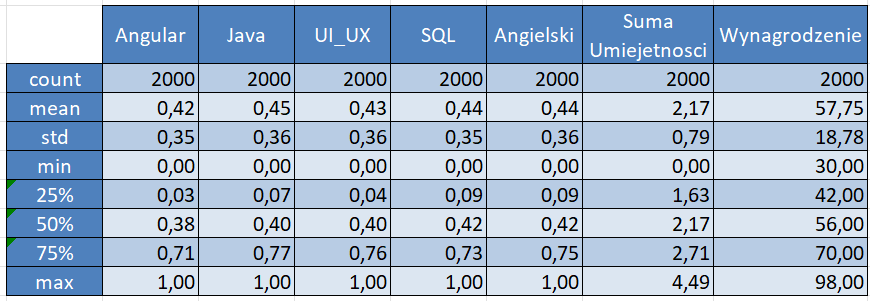
\includegraphics[width=\linewidth]{chapters/Images/analiza_tabela_all.png}
        \cprotect\caption{Tabela populacji pracowników po analizie\\ Źródło:\textit{ opracowanie własne}}
        \label{fig:tabela_analiza}
    \end{figure}

    \par Z tak wygenerowanej tabeli można wyciągnąć następujące wnioski:
    \begin{description}
        \item[Rozmiar populacji\label{itm:count}]  - Pokazuje rozmiar populacji i potwierdza, że analiza została przeprowadzona na pełnym zestawie danych.
        
        \item[Średnia\label{itm:mean}] - Średnia z każdej umiejętności wynosi od $0,42$ do $0,45$, co sugeruje, że większość pracowników posiada średni poziom umiejętności w każdej kategorii. W porównaniu do maksimum poszczególnych umiejętności, znaczna część pracowników posiada niższy o ponad połowę skali poziom umiejętności, niż maksymalny w populacji. Takie średnie są powodem dla średniej sumy pięciu umiejętności równej $2,17$. Natomiast średnia wynagrodzenia jest równa $57,75$ na godzinę, co daje dobre pojęcie o tym, jakiego wynagrodzenia średnio oczekują pracownicy tej firmy i może sugerować, że pracownicy z wyższą sumą umiejętności będą oczekiwać wyższego wynagrodzenia.
        
        \item[Odchylenie standardowe\label{itm:std}] - Odchylenie std. każdej umiejętności będące na dosyć wysokim poziomie $[0,35; 0,36]$, wskazuje na duże zróżnicowanie w poziomach opanowania poszczególnych umiejętności przez pracowników. Co za tym idzie, odchylenie std. dla sumy umiejętności wynoszące $0,79$ jest wysokie  i wskazuje na dużą zmienność w łącznym poziomie umiejętności wśród populacji pracowników firmy. Podobnie w wypadku wynagrodzenia, gdzie odchylenie std. wynosi $18,78$ będąc również na wysokim poziomie. W porównaniu do maksimum żądanego wynagrodzenia wynoszącego $98,00$, takie odchylenie sugeruje obecność dużego zróżnicowania w kwestii wynagrodzenia w populacji i może być spowodowane różnicami w umiejętnościach i sumie umiejętności.
        
        \item[Minimum\label{itm:min}] - Minimalne wartości w poszczególnych kategoriach wynoszą $0$, co dowodzi, że niektórzy pracownicy nie posiadają żadnych umiejętności w danej kategorii. Minimalne wynagrodzenie wynosi $30,00$ co nasuwa wnioski, że najmniej zarabiają pracownicy, o najmniejszej sumie umiejętności.
        
        \item[Maksimum\label{itm:max}] - Maksymalne wartości w poszczególnych kategoriach umiejętności wynoszą $1,00$, co sugeruje istnienie pracowników, którzy opanowali pewne dziedziny w pełni. Jednak można zauważyć, że w populacji nie ma pracownika, który by opanował każdą z umiejętności, gdyż maksymalna suma umiejętności wynosi $4,49$. Natomiast maksymalne wynagrodzenie wynoszące $98,00$, świadczy o obecności pracowników, którzy bardzo cenią swoja wysoką ekspertyzę. Wysoki poziom umiejętności jest ważny, jednak wysokie koszty takich pracowników, mogą ich wyeliminować z końcowego zespołu.
        
        \item[Kwartyle 25\%, 50\% i 75\%\label{itm:kwartyl}] - Kwartyle pokazują jaki rozkład mają poszczególne statystyki i pokazują rozproszenie wartości są rozproszone w populacji pracowników. 
            \begin{itemize}
                \item W kwartylu pierwszym (25\%) umiejętności są na poziomie od $0,3$ do $0,9$, co oznacza istnienie znacznej grupy pracowników o bardzo niskich umiejętnościach i ich sumie, która jest równa lub niższa $1,63$. W kwestii wynagrodzenia, w kwartylu pierwszym pracownicy nie żądają więcej niż $42,00$, co czyniłoby ich dobrymi kandydatami do zespołu, gdyby nie niska suma umiejętności.
                \item W kwartylu drugim (50\%) umiejętności mają wartości pomiędzy $0,38$ a $0,42$, co sugeruje istnienie sporej grupy pracowników o umiejętnościach zbliżonych do średniej i o sumie umiejętności wynoszącej $2,17$, która jest równa średniej sumie umiejętności. W kwestii wynagrodzenia, pracownicy z kwartylu drugiego oczekują wynagrodzenia na poziomie bardzo zbliżonym do średniej równego $56,00$. Takie dane mogą sugerować, że w kwartylu drugim znajdują się pracownicy dobrze pasujący do zespołu omawianego w problemie.
                \item Kwartyl trzeci obejmuje pracowników z umiejętnościami na poziomie poniżej około od $0,71$ do $0,76$. Wiadomo dzięki temu, że tylko 25\% pracowników ma umiejętności na wyższym poziomie niż ta grupa. Suma umiejętności w tym kwartylu wynosi $2,71$ i jest znacznie (o $0,54$) większa od średniej sumy. Wynagrodzenie natomiast wynosi $70,00$, co jest logicznym wynikiem, że większe umiejętności wiążą się z większym oczekiwanym wynagrodzeniem.
            \end{itemize}
        
    \end{description}
    \par Dzięki takie analizie, można wyciągnąć silne wnioski na temat tego, kto zostanie wybrany do zespołu i jak będą wyglądać statystyki takiego zespołu. Optymalnie wybrani pracownicy będą oczekiwali wynagrodzenia z kwartyla drugiego, co wiąże się z niższą ekspertyzą w niektórych kategoriach.
    
    \subsection{Histogramy}\label{subsec:histogramy}
    \par Histogramy przedstawiają częstotliwość występowania pracowników o danych poziomach umiejętności, wynagrodzenia czy sumy umiejętności. Oś X, przedstawia zakres poziomu umiejętności wynosi $[0, 1]$, a oś Y reprezentuje częstotliwość występowania pracowników z określonym poziomem dla danej kategorii w konkretnym zakresie. W przypadku histogramów sumy umiejętności oraz wynagrodzenia oś X przedstawia kolejno zakresy $[0, 5]$ oraz $[0, 100]$. Osie Y w tych wypadkach pozostają niezmienne. Badanie histogramów może wpłynąć na polityki wynagrodzeń oraz na strategie rozwoju firmy. Histogramy pozwolą wyłonić jakie obszary wymagają poprawy oraz pomogą w lepszym docenianiu pracowników z wyższymi umiejętnościami, promując rozwój.
    
        \subsubsection{Umiejętności w kategorii Angular}
        \begin{figure}[H]
            \centering
            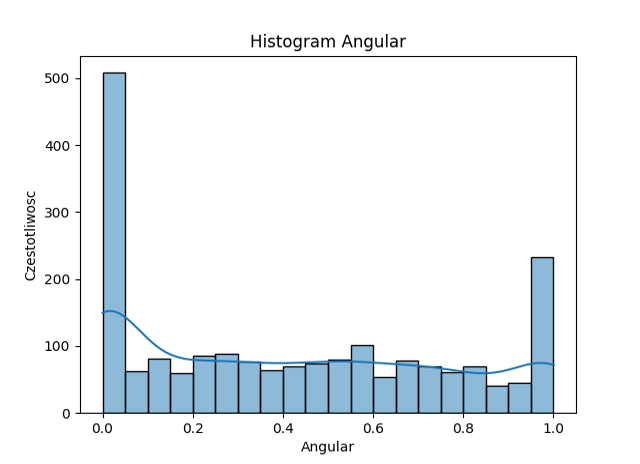
\includegraphics[width=\linewidth]{chapters/Images/hist_angular.png}
            \cprotect\caption{Histogram umiejętności w kategorii Angular\\ Źródło:\textit{ opracowanie własne}}
            \label{fig:hist_angular}
        \end{figure}

        \begin{enumerate}
            \item Występowanie najwyższych słupków przy wartościach $0$ i $1$ oznacza, że wielu pracowników (około 500 dla wartości $0$ i około 250 dla wartości $1$) posiada minimalnym lub maksymalny poziom umiejętności. Stanowi to, że około $25\%$ pracowników nie posiada umiejętności w tej kategorii, a około $12,5\%$ posiada bardzo wysoki poziom zaawansowania.
            \item Rozkład poziomu umiejętności $[0,1; 0,9]$ jest stosunkowo równomierny, z minimalną fluktuacją. Pokazuje to, że w tym przedziale umiejętności znajduje się największa część populacji (około $1250$) i jednocześnie, że mały odsetek populacji posiada średnie umiejętności w tej kategorii. Wartości zbliżone do średniej posiada około $150$ pracowników.
            \item Krzywa gęstości potwierdza obserwacje z poprzedniego punktu, mówiące o rozkładzie umiejętności w populacji, głównie w przedziale $[0,1; 0,9]$ z około $37,5\%$ populacji rozłożonej przy wartościach $0$ i $1$.
        \end{enumerate}
        
        \subsubsection{Umiejętności w kategorii Java}
        \begin{figure}[H]
            \centering
            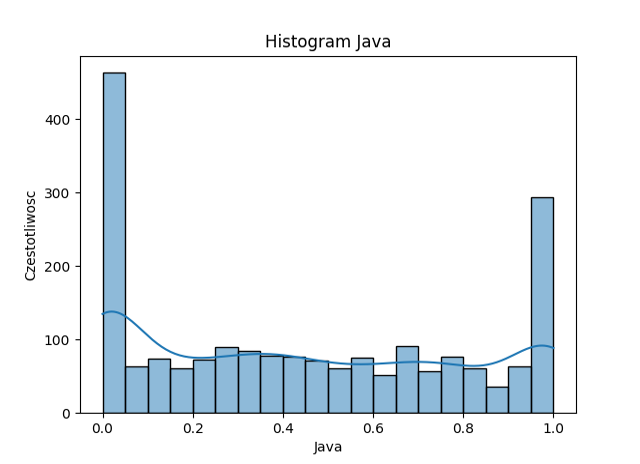
\includegraphics[width=\linewidth]{chapters/Images/hist_java.png}
            \cprotect\caption{Histogram umiejętności w kategorii Java\\ Źródło:\textit{ opracowanie własne}}
            \label{fig:hist_java}
        \end{figure}

        \begin{enumerate}
            \item Podobnie jak przy kategorii Angular najwyższe słupki występują przy wartościach $0$ i $1$ co oznacza, że wielu pracowników (około $450$ dla wartości $0$ i około $300$ dla wartości $1$) posiada tę umiejętność na poziomie równym $0$ lub $1$. Stanowi to, że około $22,5\%$ pracowników nie posiada umiejętności w tej kategorii, a około $15\%$ posiada bardzo wysoki poziom zaawansowania.
            \item Rozkład poziomu umiejętności $[0,1; 0,9]$ jest stosunkowo równomierny, z minimalną fluktuacją. Wskazuje to, że znaczna część populacji (około $1250$) posiada umiejętności w tym zakresie, a umiejętności zbliżone do średniej posiada około $170$ pracowników.
            \item Obserwacja krzywej gęstości daje takie same wnioski, mówiące o rozkładzie umiejętności w populacji, jako zdominowanej przez wartości z przedziału $[0,1; 0,9]$, a resztą skupioną przy wartościach $0$ i $1$.
        \end{enumerate}
        
        \subsubsection{Umiejętności w kategorii UI/UX}
        \begin{figure}[H]
            \centering
            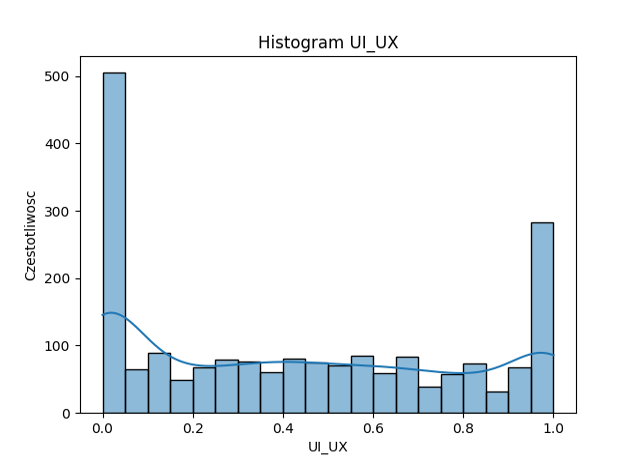
\includegraphics[width=\linewidth]{chapters/Images/hist_uiux.png}
            \cprotect\caption{Histogram umiejętności w kategorii UI/UX\\ Źródło:\textit{ opracowanie własne}}
            \label{fig:hist_uiux}
        \end{figure}

        \begin{enumerate}
            \item Bardzo zbliżone wnioski można wyczytać z histogramu kategorii UI/UX. Najwyższe słupki występują przy wartościach $0$ i $1$ co oznacza, że wielu pracowników (około $500$ dla wartości $0$ i około $300$ dla wartości $1$) posiada tę umiejętność na poziomie równym $0$ lub $1$. Dowodzi to, że około $25\%$ pracowników nie posiada umiejętności w tej kategorii, a około $15\%$ posiada bardzo wysoki poziom zaawansowania.
            \item Rozkład poziomu umiejętności $[0,1; 0,9]$ jest dosyć równomierny. Minimalna fluktuacja wskazuje, że znaczna część populacji (około $1200$) posiada umiejętności w tym zakresie, a umiejętności zbliżone do średniej posiada około $180$ pracowników. Obserwacja krzywej gęstości potwierdza te wnioski i nie wnosi nowych.
        \end{enumerate}
        
        \subsubsection{Umiejętności w kategorii SQL}
        \begin{figure}[H]
            \centering
            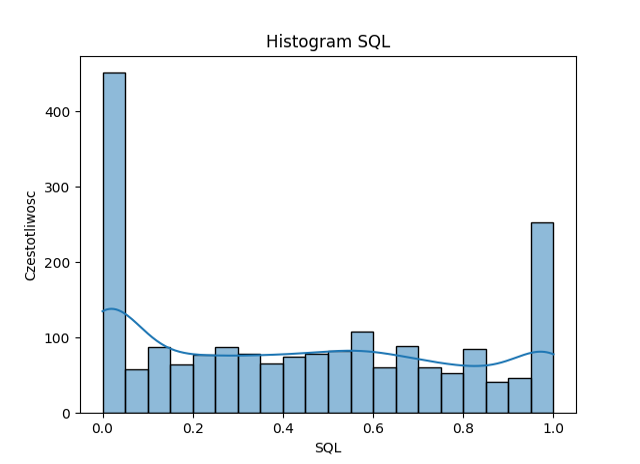
\includegraphics[width=\linewidth]{chapters/Images/hist_sql.png}
            \cprotect\caption{Histogram umiejętności w kategorii SQL\\ Źródło:\textit{ opracowanie własne}}
            \label{fig:hist_sql}
        \end{figure}

        \begin{enumerate}
            \item Histogram kategorii SQL wskazuje na podobny wzorzec jak w poprzednich przypadkach. Wysokie słupki dla wartości $0$ (około $450$ pracowników) i $1$ (około $250$ pracowników), ze znaczną częścią populacji (około $1700$ lub $65\%$ pracowników) z umiejętnościami w przedziale $[0,1; 0,9;]$. Blisko średniej znajduje się około $180$ pracowników. Krzywa gęstości potwierdza te obserwacje.
        \end{enumerate}
        
        \subsubsection{Umiejętności w kategorii Znajomość języka angielskiego}
        \begin{figure}[H]
            \centering
            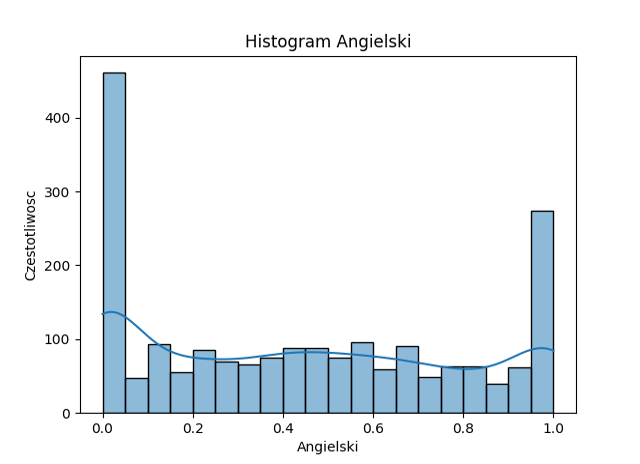
\includegraphics[width=\linewidth]{chapters/Images/hist_angielski.png}
            \cprotect\caption{Histogram umiejętności w kategorii Znajomość języka angielskiego\\ Źródło:\textit{ opracowanie własne}}
            \label{fig:hist_ang}
        \end{figure}

        \begin{enumerate}
            \item Podobnie jak w poprzednich kategoriach, najwyższe słupki dla kategorii znajomość języka angielskiego znajdują się przy wartościach $0$ (około $450$ pracowników) oraz $1$ (około $250$ pracowników). Około $1300$ pracowników ma umiejętności w przedziale od $0,1$ do $0,9$, a wartości blisko średniej posiada około $190$ pracowników. Krzywa gęstości potwierdza obserwacje dotyczącą rozkładu populacji na wykresie.
        \end{enumerate}
        
        \subsubsection{Umiejętności w kategorii Suma umiejętności}
        \begin{figure}[H]
            \centering
            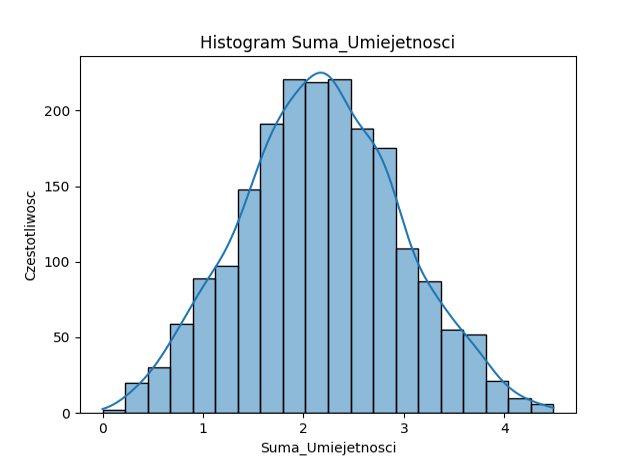
\includegraphics[width=\linewidth]{chapters/Images/hist_suma.png}
            \cprotect\caption{Histogram umiejętności w kategorii Suma umiejętności\\ Źródło:\textit{ opracowanie własne}}
            \label{fig:hist_suma}
        \end{figure}

        \begin{enumerate}
            \item Histogram dla kategorii Sumy umiejętności kształtem przypomina rozkład normalny (kształt dzwonu), co wskazuje na koncentrację pracowników około średniej sumy umiejętności, z minimalnymi przypadkami (około $80$ lub $0,04\%$ pracowników) ze skrajnie niską lub skrajnie wysoką sumą. Największa część tego zbioru (około $700$ lub $35\%$ pracowników) posiada sumę umiejętności zbliżoną do średniej. Odchylenie standardowe jest potwierdzone kształtem histogramu i potwierdza, że większość populacji ma wartość zbliżoną do średniej, a znaczna mniejszość posiada wartości skrajne. Minimum oraz maksimum również zostają odzwierciedlone na histogramie, gdyż widoczne są pojedyncze przypadki wartości minimalnych lub maksymalnych.
            \item Najwyższa częstotliwości w tej populacji występują w przedziale od $1,9$ do $2,5$, co dowodzi, że jest to najbardziej typowy poziom umiejętności w tej firmie. Częstotliwość spada niemal symetrycznie po obu stronach od średniej, co potwierdza podobieństwo do rozkładu normalnego.
            \item Łagodna krzywa gęstości również potwierdza podobieństwo do rozkładu normalnego i znikomość pracowników przy skrajnych wartościach. 
        \end{enumerate}

        \subsubsection{Umiejętności w kategorii Wynagrodzenie}
        \begin{figure}[H]
            \centering
            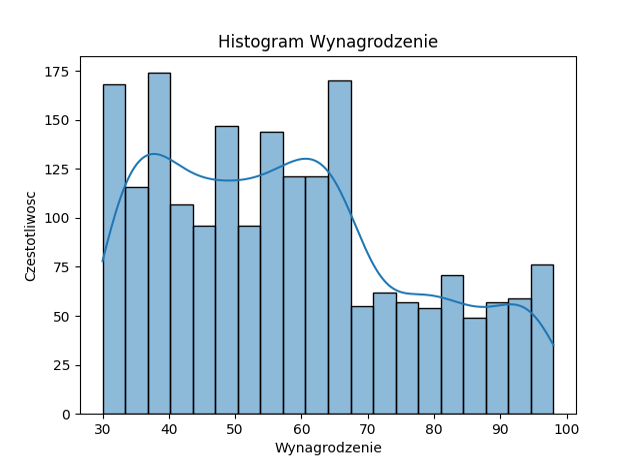
\includegraphics[width=\linewidth]{chapters/Images/hist_wynagrodzenie.png}
            \cprotect\caption{Histogram umiejętności w kategorii Wynagrodzenia\\ Źródło:\textit{ opracowanie własne}}
            \label{fig:hist_wynagrodzenie}
        \end{figure}

        \begin{enumerate}
            \item Histogram pokazuje wysokie rozproszenie kwoty wynagrodzenia na godzinę jaką otrzymują pracownicy firmy. Znaczna liczba populacji (około $460$) dostaje wynagrodzenie z przedziału $[30, 40]$ złotych/godzinę. Następnie widać wyraźny spadek dla przedziału $[40, 45]$ i nagły wzrost dla wartości około $50$. Po kolejnej drobnej fluktuacji, następuje kolejny wzrost dla drugiego wyraźnego szczytu w przedziale dla około $[55, 65]$, w którym częstotliwość wynosi około $575$. Pokazuje to, że znaczna część populacji (około $29\%$) dostaje wynagrodzenie między $55$, a $65$ złotych/godzinę co jest zgodne ze średnią. Dodatkowo odchylenie standardowe wskazuje na dużą zmienność wynagrodzenia w populacji, co jest dobrze uwidocznione na histogramie poprzez różnice w wysokościach słupków. Wyższe wynagrodzenia od $70$ do $100$ złotych na godzinie nie są już tak częste. Przedział jest trzy razy dłuższy od przedziału z najmniejszą płacą, a mieści się w nim tylko około $550$ pracowników.
            \item Krzywa gęstości pokazuje, że populacja jest głównie skoncentrowana w przedziale około $[30, 70]$ i stanowi to około $1450$ pracowników. Dodatkowo, krzywa posiada kilka szczytów co wskazuje na niejednolity rozkład. 
            \item Tendencyjnie krzywa gęstości osiąga najwyższe wartości w przedziałach $[30, 40]$ oraz $[50, 65]$ co stanowi o największej ilości pracowników zarabiających kwoty z tych przedziałów. Krzywa zalicza spadek przy wartościach większych od $70$ co dowodzi o małej części populacji zarabiającej kwoty powyżej $70$ złotych/godzinę. Długie ogony krzywej udowadniają małą liczbę pracowników zarabiające maksymalne i minimalne kwoty.
        \end{enumerate}
    
    \subsection{Macierz korelacji}\label{subsec:korelacja}
    \begin{figure}[H]
        \centering
        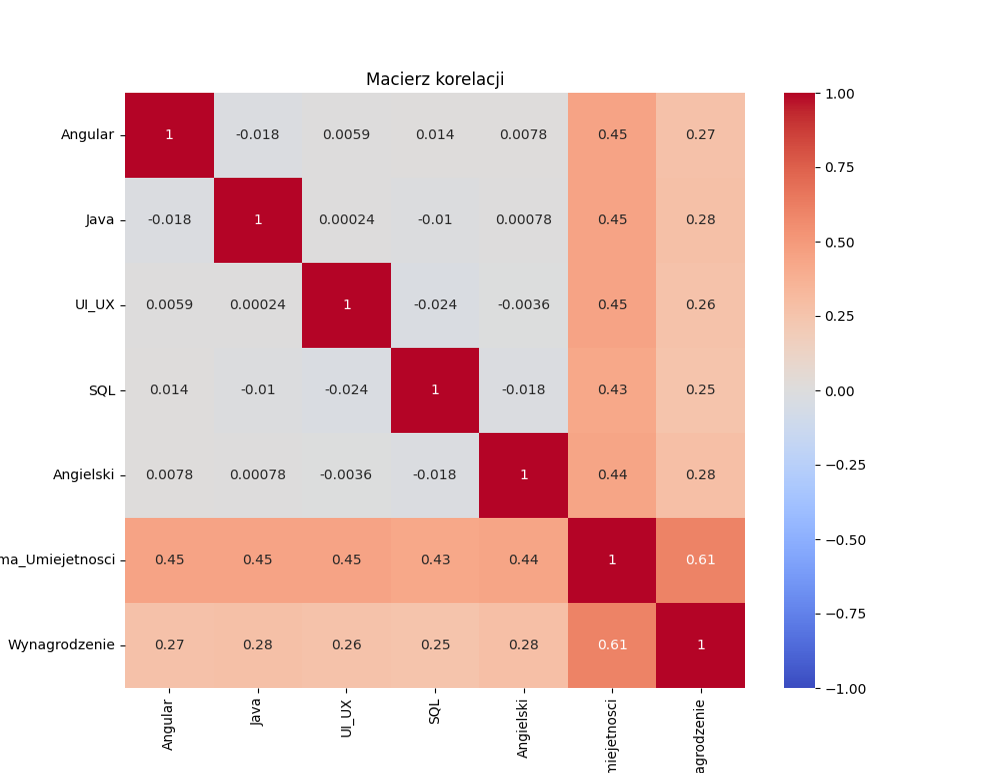
\includegraphics[width=\linewidth]{chapters/Images/korelacja.png}
        \cprotect\caption{Macierz korelacji danych\\ Źródło:\textit{ opracowanie własne}}
        \label{fig:korelacja}
    \end{figure}

    \par Do przedstawienia związków między poszczególnymi umiejętnościami, ich sumą oraz wynagrodzeniem wykorzystano macierz korelacji. Sprawdzenie, jak różne umiejętności oddziałują na siebie nawzajem oraz na sumę umiejętności i wynagrodzenie. Takie sprawdzenie pomoże ustalić, które z umiejętności mają największy wpływ na wynagrodzenie oraz jak rozwój poszczególnych umiejętności może wpłynąć na ogólny poziom kompetencji zespołu. Dzięki takiej analizie, menedżerowie mogą lepiej planować szkolenia, polityki wynagrodzeń oraz rekrutacje ze skutkiem zwiększenia efektywności i umiejętności w zespole.

    \par Związki między dwiema zmiennymi są opisane za pomocą liczb całkowitych z przedziału $[-1, 1]$, a wartości te oznaczają:
    \begin{enumerate}
        \item $1$ Oznacza dodatnią korelację; wysoka zależność między zmiennymi. W przypadku wzrostu jednej, druga też rośnie.
        \item $0$ Oznacza brak korelacji; zmienne są od siebie niezależne i nie oddziałują na siebie.
        \item $-1$ Oznacza ujemną korelację; wysoka zależność między zmiennymi. W przypadku wzrostu jednej, druga maleje.
    \end{enumerate}

    \par W przypadku korelacji między poszczególnymi umiejętnościami wartości są zawsze bliskie zeru, co oznacza, że np. posiadanie umiejętności w kategorii Angular, nie ma wpływu na poziom umiejętności SQL i na odwrót. Posiadanie umiejętności w jednej kategorii nie pomaga w zdobyciu umiejętności w innej kategorii, ale też nie utrudnia. 
    
    \par W kontekście sumy umiejętności, poszczególne umiejętności posiadają dodatnią korelację z sumą. Oznacza to, że wraz z wzrostem poszczególnych kategorii, pracownik będzie osiągać wyższą sumę umiejętności. Wpływ sumy jest też obserwowalny; gdy suma maleje, poszczególne umiejętności też maleją.

    \par Wynagrodzenie silnie koreluje z sumą umiejętności (a suma silnie koreluje z wynagrodzeniem). Pokazuje to, że wzrost wynagrodzenia bardzo często wiąże się z wysoką sumą umiejętności. Tak samo jak wysoka suma będzie wiązać się z wyższym wynagrodzeniem.

    \par Macierz korelacji pokazuje jaki wpływ mają na siebie poszczególne umiejętności oraz jak wpływają na wynagrodzenie i sumę. Dzięki takimi informacjom, menedżerowie mogą lepiej dostosować plan szkoleń w celu zwiększenia poziomu umiejętności zespołu i przewidzieć efekty jakie będzie to mieć na żądane wynagrodzenia. Dodatkowo, przy rekrutacjach będzie można ocenić jak wysokiego wynagrodzenia będzie oczekiwał pracownik w oparciu o jego umiejętności. Efektem takiego poglądu na relacje między zmiennymi będzie lepsze dostosowanie strategii przyznawania wynagrodzeń oraz dostosowanie szkoleń pod potrzeby zespołu. 
    
    \subsection{Wykres rozrzutu}\label{subsec:scatter}
    \begin{figure}[H]
        \centering
        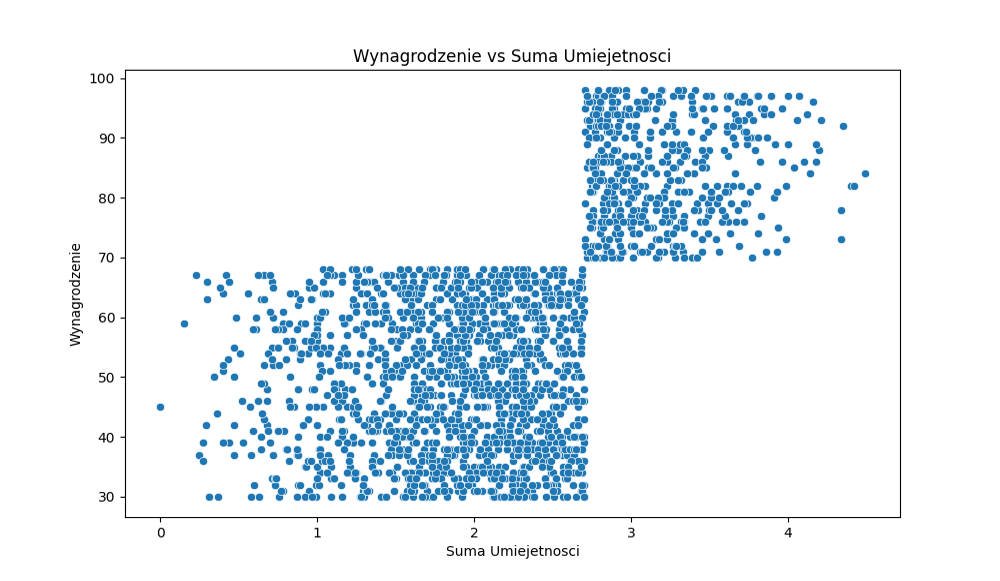
\includegraphics[width=\linewidth]{chapters/Images/rozrzut.png}
        \cprotect\caption{Wykres rozrzutu Wynagrodzenie vs Suma umiejętności\\ Źródło:\textit{ opracowanie własne}}
        \label{fig:scatter_plot}
    \end{figure}

    \par Do kolejnego etapu analizy wykorzystano wykres rozrzutu przedstawiający związek między danymi z kolumny Wynagrodzenie a danymi z kolumny Suma umiejętności. Oś X reprezentuje zakres sumy umiejętności, a analogicznie oś Y reprezentuje zakres wynagrodzeń. Punkty na wykresie oznaczają poszczególnego pracownika z populacji.

    \par Wykres jest bardzo widocznie podzielony na dwa wyraźne klastry punktów. Pierwszy i większy klaster obejmuje na osi X obszar od $0$ do około $2,7$ i na osi Y od $30$ do około $70$. Reprezentuje on część populacji, posiadającą sumę umiejętności poniżej $3$, która w efekcie zarabia w przedziale około $[30, 70]$. W tym klastrze, wynagrodzenie nie wykazuje bardzo silnej zależności od sumy umiejętności, co oznacza że nawet pracownicy z niską sumą zarabiają kwoty w górnej granicy przedziału. 

    \par W drugim klastrze znajduje się część populacji o sumie umiejętności w przedziale od około $2,7$ do $5$ i o wynagrodzeniu z przedziału około $[70, 100]$. Ten klaster pokazuje, że wyższy poziom umiejętności wiąże się z wyższym wynagrodzeniem. Można zauważyć, że nawet minimalny wzrost poziomu umiejętności ponad dolną granice tego przedziału powoduje spory wzrost wynagrodzenia. Dzieje się tak z powodu w jaki zostały wygenerowane dane; pracownicy, których suma umiejętności jest większa od trzeciego kwartyla, otrzymują losowe wynagrodzenie z przedziału $[70, 99]$. 

    \par Wykres ten można również zidentyfikować jako wykres:
    \begin{enumerate}
        \item Z silną istotnością zależności. Oznacza to, że zmienne z osi X i Y silnie na siebie oddziałują.
        \item Z liniowym rodzajem korelacji. Wraz z wzrostem wartości na osi X, wzrastają wartości na osi Y.
        \item Nieposiadający wartości odstających.
    \end{enumerate}

    \par Informacje z takiego wykresu mogą posłużyć menedżerom do opracowania lepszej polityki rozwojowej dla pracowników, która będzie nagradzać wyższe umiejętności lepszym wynagrodzeniem. Szczególnie po przekroczeniu progu (około $2,7$) wynagrodzenie zostaje znacznie zwiększone, co może silnie motywować pracowników do rozwoju swoich umiejętności. Pomoże to również w ocenie sprawiedliwości przyznawanych wynagrodzeń, mogą zdarzać się wypadki, gdy ktoś mniej uzdolniony zarabia kwotę z górnej części przedziału, a pracownik z wyższymi umiejętnościami zarabia rażąco mniej.


%<<<<<<<<<<<<<<<<<<<<<<<<<<<<<<<<<<<<<<<< ANALIZA WYNIKÓW >>>>>>>>>>>>>>>>>>>>>>>>>>>>>>>>>>>>>>>>>>>>>>>>>>>>>    
    \subsection{Interpretacja analizy wyników optymalizacji}\label{subsec:analiza_optimal}
    \par Przeanalizowane wyniki optymalizacji przez skrypt \verb|optimizer.py| zostały przeanalizowane przez \verb|analyzer.py|. Plik posiada nazwę jaką nadał mu użytkownik w momencie uruchamiania skryptu analizującego. Dane z analizy zostały podzielone na dwa arkusze. Pierwszy - \verb|Statystyki| zawiera tabele z podstawową analizą statystyczną w formie tabeli i drugi - \verb|Wykresy| zawiera histogramy, macierz korelacji i wykres rozrzutu.

    \subsection{Analiza porównawcza danych z tabeli}
    \par Tabela przedstawiona na rysunku \ref{fig:tabela_analiza_wybrani} przedstawia zestawienie statystyk obliczonych przez skrypt \verb|analyzer.py|. Struktura danych w tabeli została już opisana w przypadku populacji przy omawianiu tabeli \figrefnote{fig:tabela_analiza}.

    \begin{figure}[H]
        \centering
        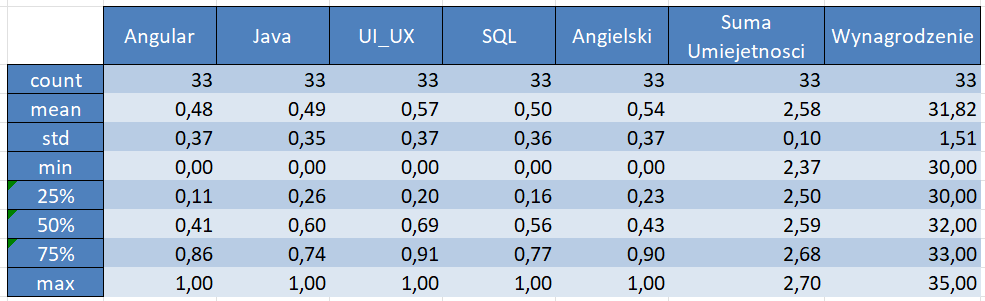
\includegraphics[width=\linewidth]{chapters/Images/analiza_tabela_wybrani.png}
        \cprotect\caption{Tabela wybranego zespołu projektowego po analizie\\ Źródło:\textit{ opracowanie własne}}
        \label{fig:tabela_analiza_wybrani}
    \end{figure}

    \par Z tak wygenerowanej tabeli można wyciągnąć następujące wnioski:
    \begin{description}
        \item[Rozmiar populacji\label{itm:count_2}]  - Pokazuje rozmiar populacji i potwierdza, że analiza została przeprowadzona na pełnym zestawie danych, otrzymanym ze skryptu \verb|optimizer.py| pracującego z zestawem danych z pliku \verb|pracownicy.csv|.
        
        \item[Średnia\label{itm:mean_2}] - Średnia z każdej umiejętności dla wybranych pracowników wynosi od $0,48$ do $0,57$. Te wartości są wyższe dla każdej kategorii w porównaniu do populacji. Podobnie w przypadku średniej sumy umiejętności, optymalny zespół posiada wyższą ogólną średnią niż populacja pracowników. Dodatkowo, wybrany zespół oczekuje średnio mniejszego wynagrodzenia, niż populacja w firmie. Wybrany zespół jest nie tylko lepszy pod kątem umiejętności, ale też wymaga mniejszych funduszy, co jest korzystne dla firmy.
        
        \item[Odchylenie standardowe\label{itm:std_2}] - Odchylenie std. dla grupy wybranych pracowników w poszczególnych umiejętnościach jest na podobnym poziomie, co u populacji. Jednak w przypadku sumy umiejętności i wynagrodzenia jest znacznie niższe ($8$ razy mniejsze dla sumy, $12$ razy mniejsze dla wynagrodzenia), co oznacza, że pracownicy w optymalnym zespole mają podobny poziom umiejętności oraz oczekują podobnego wynagrodzenia.
        
        \item[Minimum\label{itm:min_2}] - Podobnie jak w przypadku populacji, wartości poszczególnych umiejętności osiągają $0$, jednak minimum sumy umiejętności wynoszące $2,37$ jest znacznie wyższe od populacji co oznacza dużą poprawę nad minimum populacji. Minimalne wynagrodzenie wynoszące $30$ jest również takie samo jak w populacji.
        
        \item[Maksimum\label{itm:max_2}] - Dla maksimum poszczególnych kategorii, dane wynoszą tyle samo co w przypadku populacji. Jednak maksimum łącznej sumy umiejętności jest znacznie niższe niż w przypadku populacji o dokładnie $1,79$. Maksimum wynagrodzenia w optymalnym zespole wynosi $35$ złotych na godzinę.
        
        \item[Kwartyle 25\%, 50\% i 75\%\label{itm:kwartyl_2}] - Kwartyle dla optymalnego zespołu są wyższe dla prawie każdej kategorii poza wynagrodzeniem, co oznacza, że optymalny zespół posiada generalnie wyższe umiejętności i wymaga mniejszego wynagrodzenia.
            \begin{itemize}
                \item Każdy kwartyl poszczególnych umiejętności oraz sumy umiejętności jest wyższy od populacji. W kwartylu pierwszym różnice sięgają od $0,8$ do $0,19$ punktów. W drugim od $0,3$ do $0,29$ punktów, a w kwartylu trzecim jedynie umiejętności z kategorii \verb|Java| są na poziomie niższym o $0,03$. Największa różnica w kwartylu trzecim jest w kategoriach \verb|Angular, UI/UX| oraz w \verb|Angielski| i wynosi $0,15$. Suma umiejętności w trzecim kwartylu jest niewiele niższa o $0,03$.
                \item Wynagrodzenie pozostaje niższe w trzecim i drugim kwartylu kolejno różniące się o $37$ złotych i $24$ złote.
            \end{itemize}
        
    \end{description}
    
    \par Porównanie wyników z analizy populacji oraz analizy optymalnego zespołu pokazuje, że mimo ogólnie lepszych statystyk, optymalny zespół może nie posiadać pracowników z bardzo wysoką generalną ekspertyzą. Warunek utrzymania niskiego kosztu pozwolił dobrać pracowników, nieoczekujących wysokiego wynagrodzenia, ale kosztem eksperckich umiejętności w zespole.
    
    \subsection{Histogramy}
    \par Histogramy przedstawiają częstotliwość występowania pracowników o danych poziomach umiejętności, wynagrodzenia czy sumy umiejętności. Podobne wykresy zostały opisane wcześniej i następująca analiza będzie porównywać wyniki do analizy przeprowadzonej w sekcji \refnote{subsec:histogramy}.
    
        \subsubsection{Umiejętności w kategorii Angular optymalnego zespołu}
        \begin{figure}[H]
            \centering
            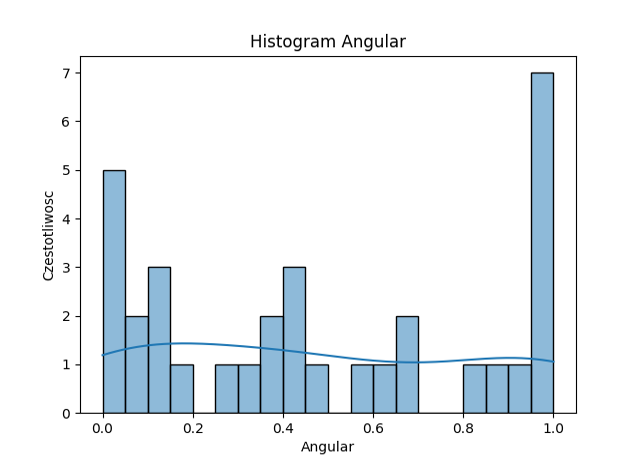
\includegraphics[width=\linewidth]{chapters/Images/hist_angular_optimal.png}
            \cprotect\caption{Histogram umiejętności w kategorii Angular dla optymalnego zespołu\\ Źródło:\textit{ opracowanie własne}}
            \label{fig:hist_angular_optimal}
        \end{figure}

        \begin{enumerate}
            \item Występowanie najwyższych słupków przy wartościach $0$ i $1$ jest podobne do tego przy populacji, jednak w optymalnym zespole $21\%$ pracowników posiada pełną ekspertyzę w tej kategorii, a tylko $15\%$ nie posiada żadnej wiedzy.
            \item Rozkład poziomu umiejętności $[0,1; 0,9]$ jest bardziej zróżnicowany niż ten populacji. Widoczne są wyraźne szczyty przy $0,2$, $0,4$ i $0,6$ co sugeruje, że optymalny zespół posiada bardziej zróżnicowany poziom umiejętności, ale generalnie na wyższym poziomie. Ponad połowa wybranego zespołu ($18$) posiada umiejętności wyższe niż średnia populacji.
            \item Krzywa gęstości potwierdza obserwacje z poprzedniego punktu, ale jest bardziej płaska niż dla populacji, potwierdzając większe zróżnicowanie w poziomie umiejętności.
        \end{enumerate}
        
        \par Z histogramu można wywnioskować, że optymalny zespół posiada generalnie wyższy poziom umiejętności w kategorii Angular od populacji. Nie oznacza to jednak, że każdy członek zespołu posiada ekspertyzę w tym zakresie, gdyż w zespole znajdują się też pracownicy bez żadnej wiedzy w danym temacie. Można zakładać, że optymalizacja przyniosła pożądane efekty.
        
        \subsubsection{Umiejętności w kategorii Java optymalnego zespołu}
        \begin{figure}[H]
            \centering
            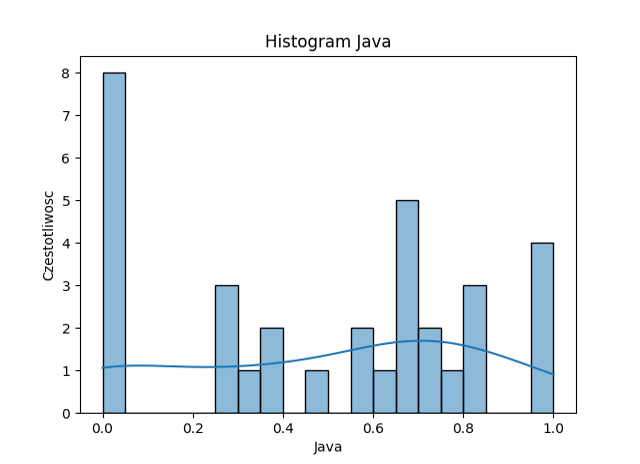
\includegraphics[width=\linewidth]{chapters/Images/hist_java_optimal.png}
            \cprotect\caption{Histogram umiejętności w kategorii Java dla optymalnego zespołu\\ Źródło:\textit{ opracowanie własne}}
            \label{fig:hist_java_optimal}
        \end{figure}

        \begin{enumerate}
            \item Najwyższe słupki na histogramie umiejętności z kategorii Java znajdują się przy punktach $0$, $1$ oraz około przedziału $[6,5; 0,7]$. Umiejętności w tej kategorii nie posiada ośmiu pracowników, natomiast ekspertyzę powyżej średniej optymalnego zespołu posiada $18$ pracowników, w tym $4$ posiada wiedzę na poziomie eksperta. Jest to znaczy wyższy poziom wiedzy od średniej populacji.
            \item Krzywa gęstości jest generalnie płaska, ze szczytami około $0,6$ oraz $1$. Taka krzywa, może sugerować sporą różnorodność w zespole w tej kategorii i ogólnie wyższy poziom umiejętności niż dla populacji.
        \end{enumerate}

        \par Umiejętności z kategorii Java są generalnie wyższe od średniej populacji, ale nie brakuje zróżnicowania w zespole. Znajdują się w nim i pracownicy, których można określać ekspertami w tej kategorii oraz pracownicy z wiedzą znikomą. Widać zamierzone efekty optymalizacji.
        
        \subsubsection{Umiejętności w kategorii UI/UX optymalnego zespołu}
        \begin{figure}[H]
            \centering
            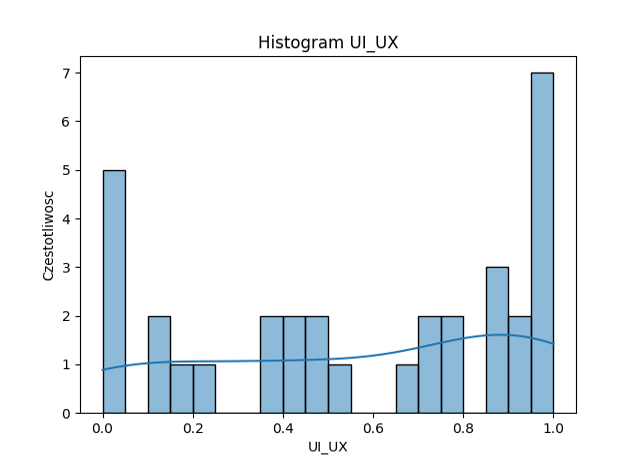
\includegraphics[width=\linewidth]{chapters/Images/hist_uiux_optimal.png}
            \cprotect\caption{Histogram umiejętności w kategorii UI/UX dla optymalnego zespołu\\ Źródło:\textit{ opracowanie własne}}
            \label{fig:hist_uiux_optimal}
        \end{figure}

        \begin{enumerate}
        \item Histogram kategorii UI/UX wykazuje, że poziom umiejętności $1$ oraz $0$ osiągnęło kolejno $7$ oraz $5$ pracowników. Ponownie pojawia się przewaga pracowników na poziomie eksperckim, co nie było obecne w populacji, w której nad ekspertami, przeważały osoby z brakiem jakiejkolwiek wiedzy w danej kategorii. Poza dwoma głównymi szczytami, na wykresie nie przebijają się inne znaczące szczyty. Ogólny rozkład w przedziale $[0,1; 0,9]$ jest równomierny, jednak ponad połowa wybranych pracowników ($18$) ma umiejętności wyższe od średniej populacji.
        \item Krzywa gęstości jest generalnie płaska, z lekkim wzrostem ku końcowi przedziału, co sugeruje równomierne rozłożenie umiejętności oraz przeważającą liczbę pracowników o poziomie wyższym od $0,5$ i średniej populacji.
        \end{enumerate}

        \par Zróżnicowanie umiejętności w kategorii UI/UX i przewaga umiejętności na poziomie wyższym od średniej populacji potwierdza działanie modelu, który przy niskim koszcie dobrał wysoce wykwalifikowany zespół.
        
        \subsubsection{Umiejętności w kategorii SQL optymalnego zespołu}
        \begin{figure}[H]
            \centering
            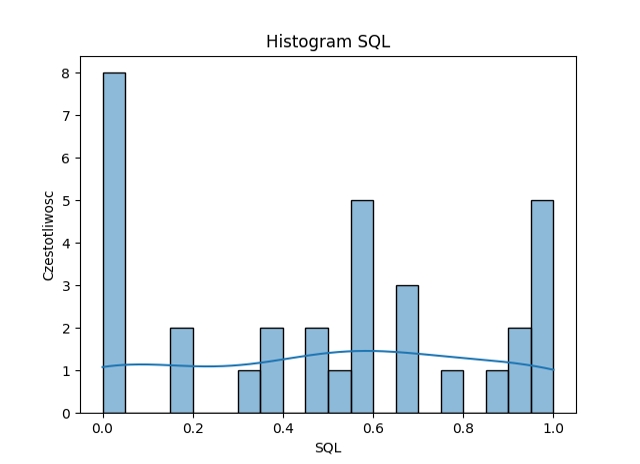
\includegraphics[width=\linewidth]{chapters/Images/hist_sql_optimal.png}
            \cprotect\caption{Histogram umiejętności w kategorii SQL dla optymalnego zespołu\\ Źródło:\textit{ opracowanie własne}}
            \label{fig:hist_sql_optimal}
        \end{figure}

        \begin{enumerate}
            \item Najwyższe słupki są dla wartości $0$, $1$ oraz $0,6$ i stanowią kolejno $8$. $5$ i $5$ pracowników z optymalnego zespołu. Mimo dużego odsetku osób bez żadnej wiedzy (około $24\%$) zespół nadal posiada wysoki poziom wiedzy w zakresie SQL. Umiejętności ponad średnią populacji posiada $17$ pracowników co stanowi ponad połowę tego zespołu. Znaczna część tego zespołu posiada odpowiedni poziom ekspertyzy, żeby z powodzeniem wykonać powierzone zadania.
            \item Krzywa gęstości potwierdza obserwacje i wskazuje na duże zróżnicowanie w zespole, pojawiają się w nim zarówno osoby bez umiejętności, eksperci oraz osoby z umiejętnościami wyższymi niż średnie.
        \end{enumerate}

        \par Przeważające umiejętności na poziomie wyższym od średniej populacji sugerują, że i w tej kategorii model dokonał poprawnej optymalizacji.
        
        \subsubsection{Umiejętności w kategorii Znajomość języka angielskiego optymalnego zespołu}
        \begin{figure}[H]
            \centering
            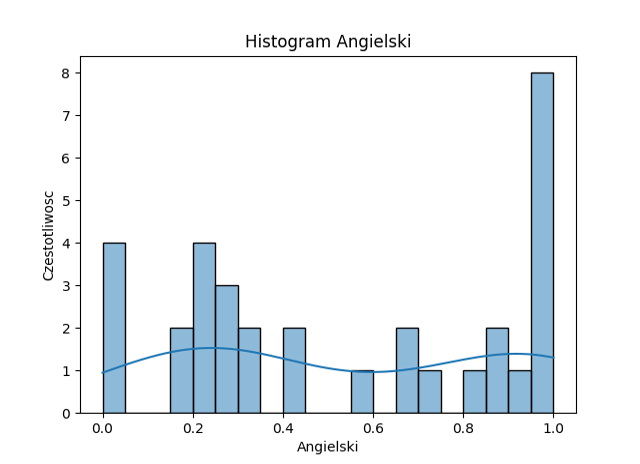
\includegraphics[width=\linewidth]{chapters/Images/hist_ang_optimal.png}
            \cprotect\caption{Histogram umiejętności w kategorii Znajomość języka angielskiego dla optymalnego zespołu\\ Źródło:\textit{ opracowanie własne}}
            \label{fig:hist_ang_optimal}
        \end{figure}

        \begin{enumerate}
            \item Dwa razy wyższy słupek symbolizujący osoby z perfekcyjną znajomością języka angielskiego, niż tego symbolizującego osoby bez żadnej wiedzy. Mimo tego, $17$ pracowników zna język angielski na poziomie niższym od średniej populacji, co nie jest zadowalające.
            \item Krzywa wskazuje na zrównoważony rozkład umiejętności pośród pracowników, ze szczytem w okolicach przedziału $[0,2; 0,3]$ i w okolicach $[0,9; 1]$.
        \end{enumerate}

        \par Mimo niezadowalającej przewagi pracowników z poziomem języka angielskiego niższym niż średnia populacji, nie jest to krytyczna umiejętność, która nie pozwala zespołowi spełnić zadania.
        
        \subsubsection{Umiejętności w kategorii Suma umiejętności optymalnego zespołu}
        \begin{figure}[H]
            \centering
            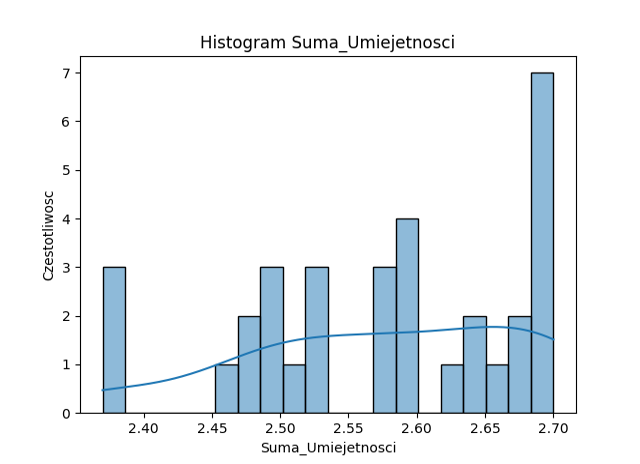
\includegraphics[width=\linewidth]{chapters/Images/hist_suma_optimal.png}
            \cprotect\caption{Histogram umiejętności w kategorii Suma umiejętności dla optymalnego zespołu\\ Źródło:\textit{ opracowanie własne}}
            \label{fig:hist_suma_optimal}
        \end{figure}

        \begin{enumerate}
            \item Najwyższym słupkiem jest ten z poziomem sumy umiejętności w okolicach $2,70$, co wskazuje na ogólnie wysoki poziom sumarycznych umiejętności zespołu. Tych siedmiu pracowników niemal posiada tak wysoka sumę umiejętności jak kwartyl trzeci populacji i znacznie przewyższa średnią populacji o $0,53$ punktów.
            \item Krzywa sugeruje znaczący wzrost sumy umiejętności od około $2,45$, co stanowi o dużej gęstości pracowników, których sumaryczne umiejętności przewyższają nad średni populacji o przynajmniej $0,25$ i więcej.
        \end{enumerate}

        \par Suma umiejętności jest większa od średniej populacji nawet w swoim minimum, co oznacza dużą poprawę poziomu umiejętności nad całą populacją. Model dokonał poprawnych wyborów co do członków zespołu w trakcie optymalizacji pod minimalny poziom umiejętności.

        \subsubsection{Umiejętności w kategorii Wynagrodzenie optymalnego zespołu}
        \begin{figure}[H]
            \centering
            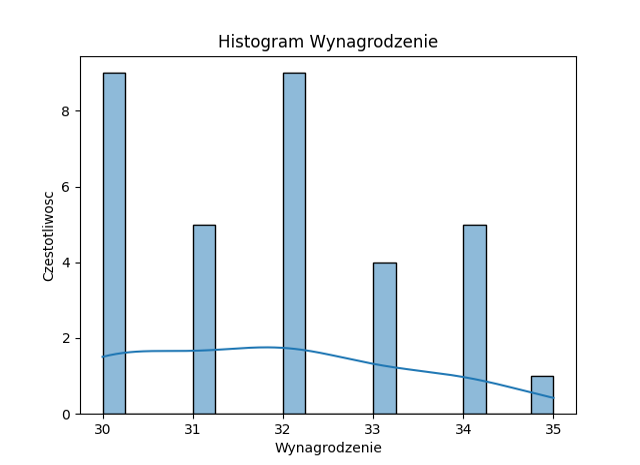
\includegraphics[width=\linewidth]{chapters/Images/hist_wynagrodzenie_optimal.png}
            \cprotect\caption{Histogram umiejętności w kategorii Wynagrodzenia dla optymalnego zespołu\\ Źródło:\textit{ opracowanie własne}}
            \label{fig:hist_wynagrodzenie_optimal}
        \end{figure}

        \begin{enumerate}
            \item Najwyższe słupki znajdują się na wartościach $30$ oraz $32$ (złotych na godzinę). Oznacza to, że w wybranym zespole prawie połowa wybranych ($16$ lub $48\%$) pracowników zarabia stawkę minimalną pod kątem populacji lub bliską minimalnej. Jest tylko jeden pracownik, który zarabia najwięcej a jego zarobki nie przekraczają średniej populacji.
            \item Krzywa gęstości wskazuje na zagęszczenie pracowników w przedziale od $30$ do $32$ z następującym spadkiem. Można z tego wywnioskować, że wynagrodzenie w tym zespole jest wyjątkowo niskie w stosunku do danych z populacji.
        \end{enumerate}
        
        \par Dane z histogramu kategorii Wynagrodzenie ponownie potwierdzają działanie i sukces modelu w optymalizacji zespołu projektowego pod ograniczeniem budżetu oraz umiejętności zespołu.
    
    \subsection{Macierz korelacji}
    \begin{figure}[H]
        \centering
        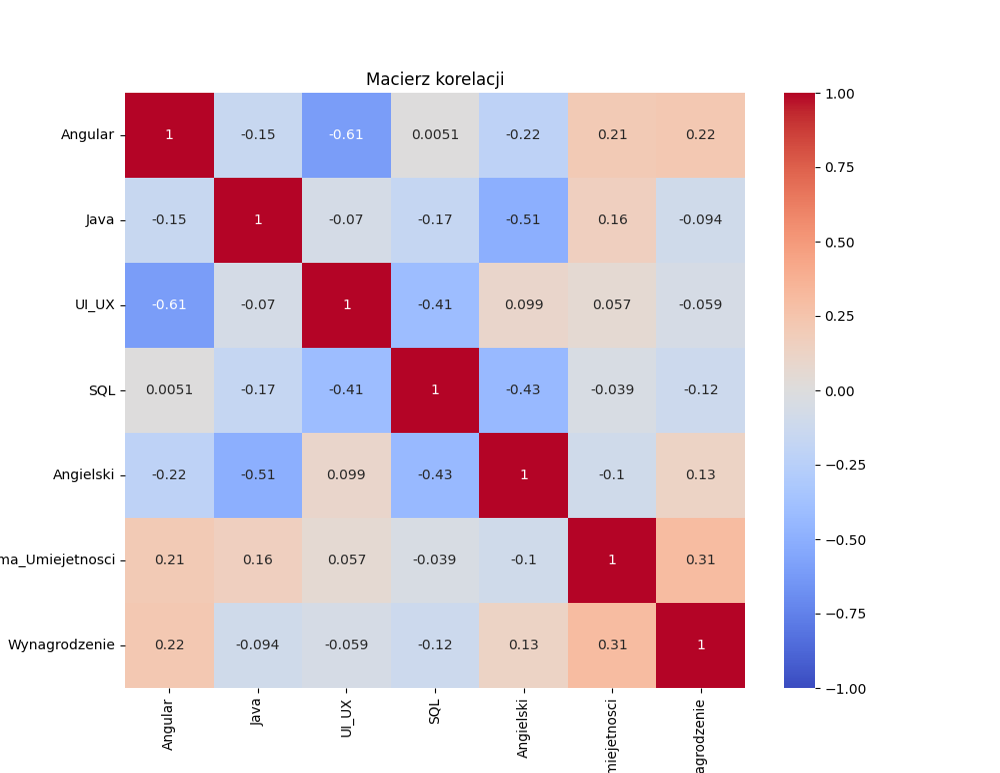
\includegraphics[width=\linewidth]{chapters/Images/korelacja_optimal.png}
        \cprotect\caption{Macierz korelacji danych\\ Źródło:\textit{ opracowanie własne}}
        \label{fig:korelacja_optimal}
    \end{figure}

    \par Ponownie wykorzystano macierz korelacji do przedstawienia związków między poszczególnymi umiejętnościami, ich sumą, a wynagrodzeniem. Analiza macierzy ma pomóc w ustaleniu czy dobór optymalnego zespołu jest skuteczniejszy dzięki niektórym korelacjom między umiejętnościami. Znaczenie wartości na macierzy zostało opisane w sekcji \refnote{subsec:korelacja}.

    \par W przypadku korelacji między poszczególnymi umiejętnościami wartości są zawsze bliskie zeru lub ujemne, a co za tym idzie nie oddziałują na siebie albo oddziałują na siebie negatywnie. W praktyce oznacza to, że posiadanie umiejętności np. z kategorii Angular nie oddziałuje na umiejętności z kategorii SQL (korelacja na poziomie $0,0051$) i na odwrót. Negatywna korelacja między kategorią Angular i kategorią UI/UX oznacza, że posiadanie wysokich umiejętności w jednym wiąże się z posiadaniem niskich umiejętności w drugim (korelacja na poziomie $-0,61$). W macierzy korelacji populacji, poszczególne umiejętności nie oddziaływały na siebie prawie w ogóle.
    
    \par W kontekście sumy umiejętności, poszczególne umiejętności posiadają głównie dodatnią lub bliską zeru korelację z sumą. Wraz ze wzrostem poziomu umiejętności, ekspertyza w innych kategoriach wzrasta lub pozostaje bez zmian. Wskazuje to na wzrost sumy wraz z ze wzrostem poszczególnych umiejętności, ale także i spadek. W przypadku populacji, suma silnie korelowała z każdą z kategorii umiejętności co oznaczało gwałtowne wzrosty oraz spadki.

    \par Wynagrodzenie silnie koreluje z sumą umiejętności, ale nie tak mocno jak w przypadku populacji. W populacji pracowników, wyższa suma umiejętności w wielu przypadkach wiązała się z wysokim wynagrodzeniem, w przeciwieństwie do optymalnego zespołu. Pokazuje to, że mimo wzrostu sumy umiejętności, w optymalnym zespole zmiany w oczekiwanym wynagrodzeniu nie są tak gwałtowne.

    \par Analiza porównawcza macierzy korelacji optymalnego zespołu w porównaniu z macierzą populacji ukazuje pewne tendencje w populacji, które zostały uwidocznione dopiero po ich zestawieniu. Mianowicie w populacji wyższy poziom umiejętności był silnie związanym ze wzrostem wynagrodzenia, gdzie w optymalnym zespole wymagane podwyżki są stosunkowo niskie. Również w populacji nie był widoczny wpływ posiadania wiedzy z jednej kategorii na inne. W przypadku optymalnego zespołu te wpływy są nieco bardziej widoczne i można zauważyć przeważnie negatywne oddziaływanie umiejętności na siebie.
    
    \subsection{Wykres rozrzutu}
    \begin{figure}[H]
        \centering
        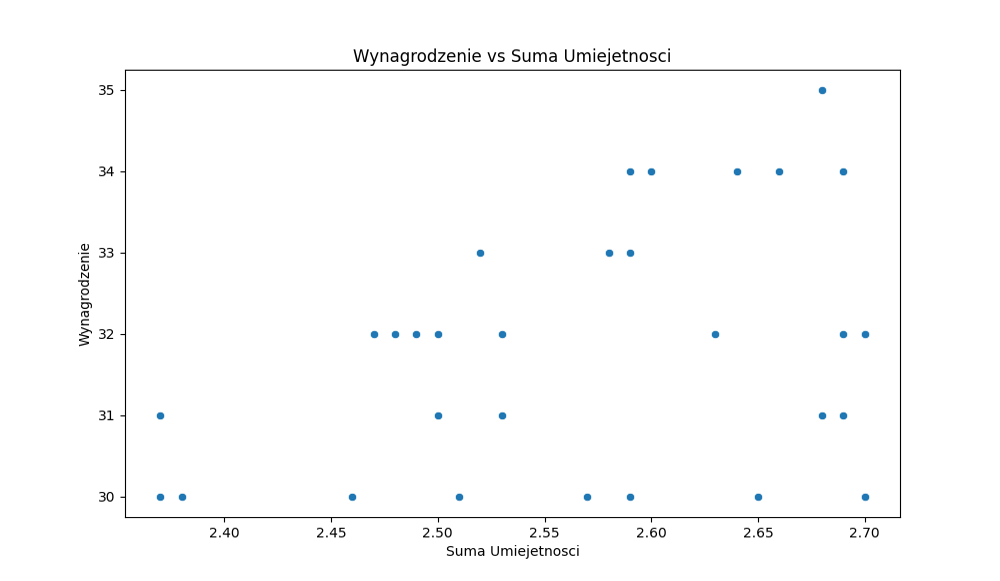
\includegraphics[width=\linewidth]{chapters/Images/rozrzut_optimal.png}
        \cprotect\caption{Wykres rozrzutu Wynagrodzenie vs Suma umiejętności\\ Źródło:\textit{ opracowanie własne}}
        \label{fig:scatter_plot_optimal}
    \end{figure}

    \par Ostatnia część analizy bazuje na wykresie rozrzutu przedstawiającego stosunek sumy umiejętności do wynagrodzenia w optymalnym zespole. Oś X przedstawia sumę umiejętności a oś Y wynagrodzenie. Punkty na wykresie to każdy z pracowników w optymalnym zespole.

    \par Wykres został bardzo widocznie podzielony prawie "na pół". Jedyny klaster na wykresie obejmuje obszar na osi X od $2,4$ do $2,7$ i na osi Y obszar od $30$ do $35$. Nie jest widoczna silna zależność między sumą umiejętności, a wynagrodzeniem, co sugeruje, że wybrani pracownicy posiadają wysoką sumę umiejętności, której stosunek do wynagrodzenia jest minimalny. Nie zaobserwowano również żadnej tendencji wskazującej na znaczy wzrost wynagrodzenia względem sumy umiejętności. W zestawieniu z wykresem rozrzutu populacji, można stwierdzić że pracownicy optymalnego zespołu "mieszczą się" w klastrze pierwszy wykresu rozrzutu populacji (Wykres rozrzutu populacji \figrefnote{fig:scatter_plot}).

    \par Wykres ten można również zidentyfikować jako wykres:
    \begin{enumerate}
        \item Z umiarkowaną istotnością zależności. Oznacza to, że zmienne z osi X i Y oddziałują na siebie, ale nie w silny sposób.
        \item Z liniowym rodzajem korelacji. Wraz z wzrostem wartości na osi X, wzrastają wartości na osi Y.
        \item Nieposiadający wartości odstających. Punkty są skoncentrowane w ramach jednego klastra i można stwierdzić brak wartości odstających.
    \end{enumerate}

    \par Informacje z takiego wykresu wskazują na skuteczność modelu optymalizacyjnego przy wyborze optymalnego zespołu projektowego. Model ograniczył swoje wybory do pracowników o wysokiej sumie umiejętności i niskich oczekiwaniach finansowych. Jednorodność klastra może sugerować, większe podobieństwo między pracownikami pod względem umiejętności.
